\documentclass{article}

% Anonymous NeurIPS 2026 main-track submission.
\usepackage{neurips_2026}
% Camera ready: \usepackage[main,final]{neurips_2026}
% Preprint:     \usepackage[preprint]{neurips_2026}

\usepackage[utf8]{inputenc}
\usepackage[T1]{fontenc}
\usepackage{hyperref}
\hypersetup{hidelinks}
\usepackage{url}
\usepackage{algorithm}
\usepackage{algpseudocode}
\usepackage{booktabs}
\usepackage{microtype}
\usepackage{xcolor}
\usepackage{graphicx}
\usepackage{amsmath}
\usepackage{amssymb}
\usepackage{mathtools}

\newcommand{\model}{\textsc{ReGRow}}
\newcommand{\RT}{\textsc{RT}}
\newcommand{\fkp}{\mathsf{f2p}}
\newcommand{\pkf}{\mathsf{p2f}}
\newcommand{\RR}{\mathbb{R}}
\newcommand{\ind}{\mathbb{I}}
\newcommand{\concat}{\mathbin\Vert}
\newcommand{\relu}{\operatorname{ReLU}}

\newcommand{\mainAUROC}{70.0}
\newcommand{\mainParams}{2.78M}
\newcommand{\wideAUROC}{71.5}
\newcommand{\wideParams}{22M}

\title{ReGRow: Relation-Guided Row-Graph Transfer for Entity Classification on Unseen Relational Databases}

\author{%
  Zhang Rongchuan \\
  Institute for Artificial Intelligence \\
  \texttt{anonymous@example.com}
}

\begin{document}
\maketitle

\begin{abstract}
% Relational databases vary in their schemas, table identities, and PK--FK
% relations, making it difficult for a model trained on one collection of
% databases to generalize to an unseen database.  We present \model{}, a compact
% graph architecture for cross-database entity classification.  

% \model{} consists of three main components. A context module collects a bounded, temporally valid neighborhood around each query and aggregates heterogeneous cell values into row representations. A relation-guidance module constructs a query-conditioned graph from the local PK--FK structure and infers relation representations without learned schema-specific identifiers. A row-reasoning module uses these representations to guide message passing between rows, followed by a shared classifier for entity prediction.

% --------------------------------------------------
% Relational databases vary in their schemas, table identities, and PK-FK relations, making it difficult for a model trained on one collection of databases to generalize to an unseen database. Recent relational foundation models have demonstrated cross-database transfer, motivating us to explore compact models that preserve relation-specific computation and exploit task context for prediction. We present \model{}, a model for cross-database entity classification that combines structurally induced relation representations, compact row-level reasoning, and context-aware candidate scoring.
% \model{} consists of three main components. A context module collects a bounded, temporally valid neighborhood around each query and uses shared encoders to aggregate heterogeneous cell values into compact row representations. A relation-guidance module constructs a query-conditioned graph from the local PK–FK structure and uses operators shared across databases to infer relation representations on unseen schemas, without learned schema-specific identifiers. A row-reasoning module uses these representations to guide message passing between rows, aggregates labeled context into class-candidate nodes, and applies a shared scorer to query–candidate pairs for entity prediction.
% Across ten binary RelBench tasks in a leave-database-out evaluation, \model{} achieves 70.0 macro AUROC with 2.78M trainable parameters, providing competitive accuracy with substantially fewer parameters than recent neural baselines.
% These results indicate that structure-induced relation representations offer a compact route to competitive cross-database transfer.

Cross-dataset entity classification on relational databases asks a model trained on multiple databases to predict entity labels in an unseen database without updating its parameters.
Existing models for this task rely on large attention-based architectures that learn from data which parts of the relational context matter.
Graph neural networks are far more compact because the relational structure itself determines how they aggregate information, but they are typically trained for a single schema.
The core challenge is to retain this efficiency without parameters specific to any database.
We present \model{}, a lightweight graph neural network in which the database structure, rather than learned attention, determines how information is aggregated, and whose parameters are tied only to roles that all databases share, never to particular tables, relations or tasks.
Specifically, \model{} (i) encodes records of any table with one shared encoder and passes messages along primary--foreign key links with two edge types common to all databases, so that computation scales with records rather than cells; (ii) replaces relation-specific weights with relation representations derived from a graph over foreign-key relations, in which relations sharing a table are adjacent; and (iii) replaces task-specific output heads by connecting records with known labels to one node per class and scoring the target against these nodes, with each timestamped record encoded by its time relative to the prediction.
With only \mainParams{} parameters, \model{} achieves \mainAUROC{} macro AUROC on ten binary classification tasks from RelBench under leave-database-out transfer, and accuracy improves with width, reaching \wideAUROC{} at \wideParams{} parameters.
\end{abstract}

% % \section{Introduction}
% % \label{sec:introduction}

% % Relational databases support predictive decisions in commerce, finance, science, and online platforms. The evidence for one prediction is rarely contained in one row: customer churn may depend on transactions and products, while a race outcome may depend on drivers, constructors, and earlier results; in both cases, only information available before the prediction time may be used. Relational Deep Learning (RDL) represents rows as nodes and primary--foreign key (PK--FK) references as edges, replacing hand-engineered join-and-aggregate pipelines with learned relational models \citep{fey2024rdl}.  RelBench makes such temporal entity-prediction problems reproducible across real databases \citep{robinson2024relbench}.  Yet a new database or prediction target still commonly starts another supervised cycle: collect labels, optimize and validate a schema-specific model, and maintain a new deployment.  Reusing one model across databases would amortize this cost and enable prediction when target labels, compute, or deployment time are limited.

% % Cross-database transfer must balance relation specificity with schema variation. Table names and PK--FK identities are local to each database, although the structural roles they express often recur.  Consider Formula~1: both 
% % \texttt{Results}$\rightarrow$\texttt{Drivers} and 
% % \texttt{Results}$\rightarrow$\texttt{Races} are child-to-parent links, but one connects an outcome to who produced it and the other to the event in which it occurred (Figure~\ref{fig:architecture}).  Without relation-specific representations, a schema-independent row GNN cannot explicitly distinguish the roles of different database relations.  Assigning a learned embedding to every relation restores this specificity, but binds the model to the training schema and leaves relations in an unseen schema undefined.  Cross-database transfer therefore requires a third option: construct relation-specific representations on a new schema without binding model parameters to its relation identities.

% % Existing approaches make different choices in this tradeoff.  Row-based RDL models such as RelGNN~\citep{chen2025relgnn}, RelGT~\citep{dwivedi2026relgt}, and Griffin~\citep{wang2025griffin} preserve
% % explicit database structure and support compact structural computation, but their principal downstream protocols optimize parameters for the target task. Recent cross-database and relational in-context approaches instead reuse parameters across schemas through cell-token representations in RT~\citep{ranjan2026rt}, synthetic schema variation in
% % PluRel~\citep{kothapalli2026plurel}, column-preserving encoding in
% % RDBLearn~\citep{xu2026rdblearn}, or hierarchical row and column representations
% % in KumoRFM-2~\citep{hudovernik2026kumorfm2}.  These systems demonstrate reusable
% % prediction across databases while making different choices about representation granularity and contextual label access.  These alternatives motivate a compact row-level design that constructs relation-specific
% % representations for the current schema using parameters shared across databases.

% % \begin{figure*}[t]
% %   \centering
% %   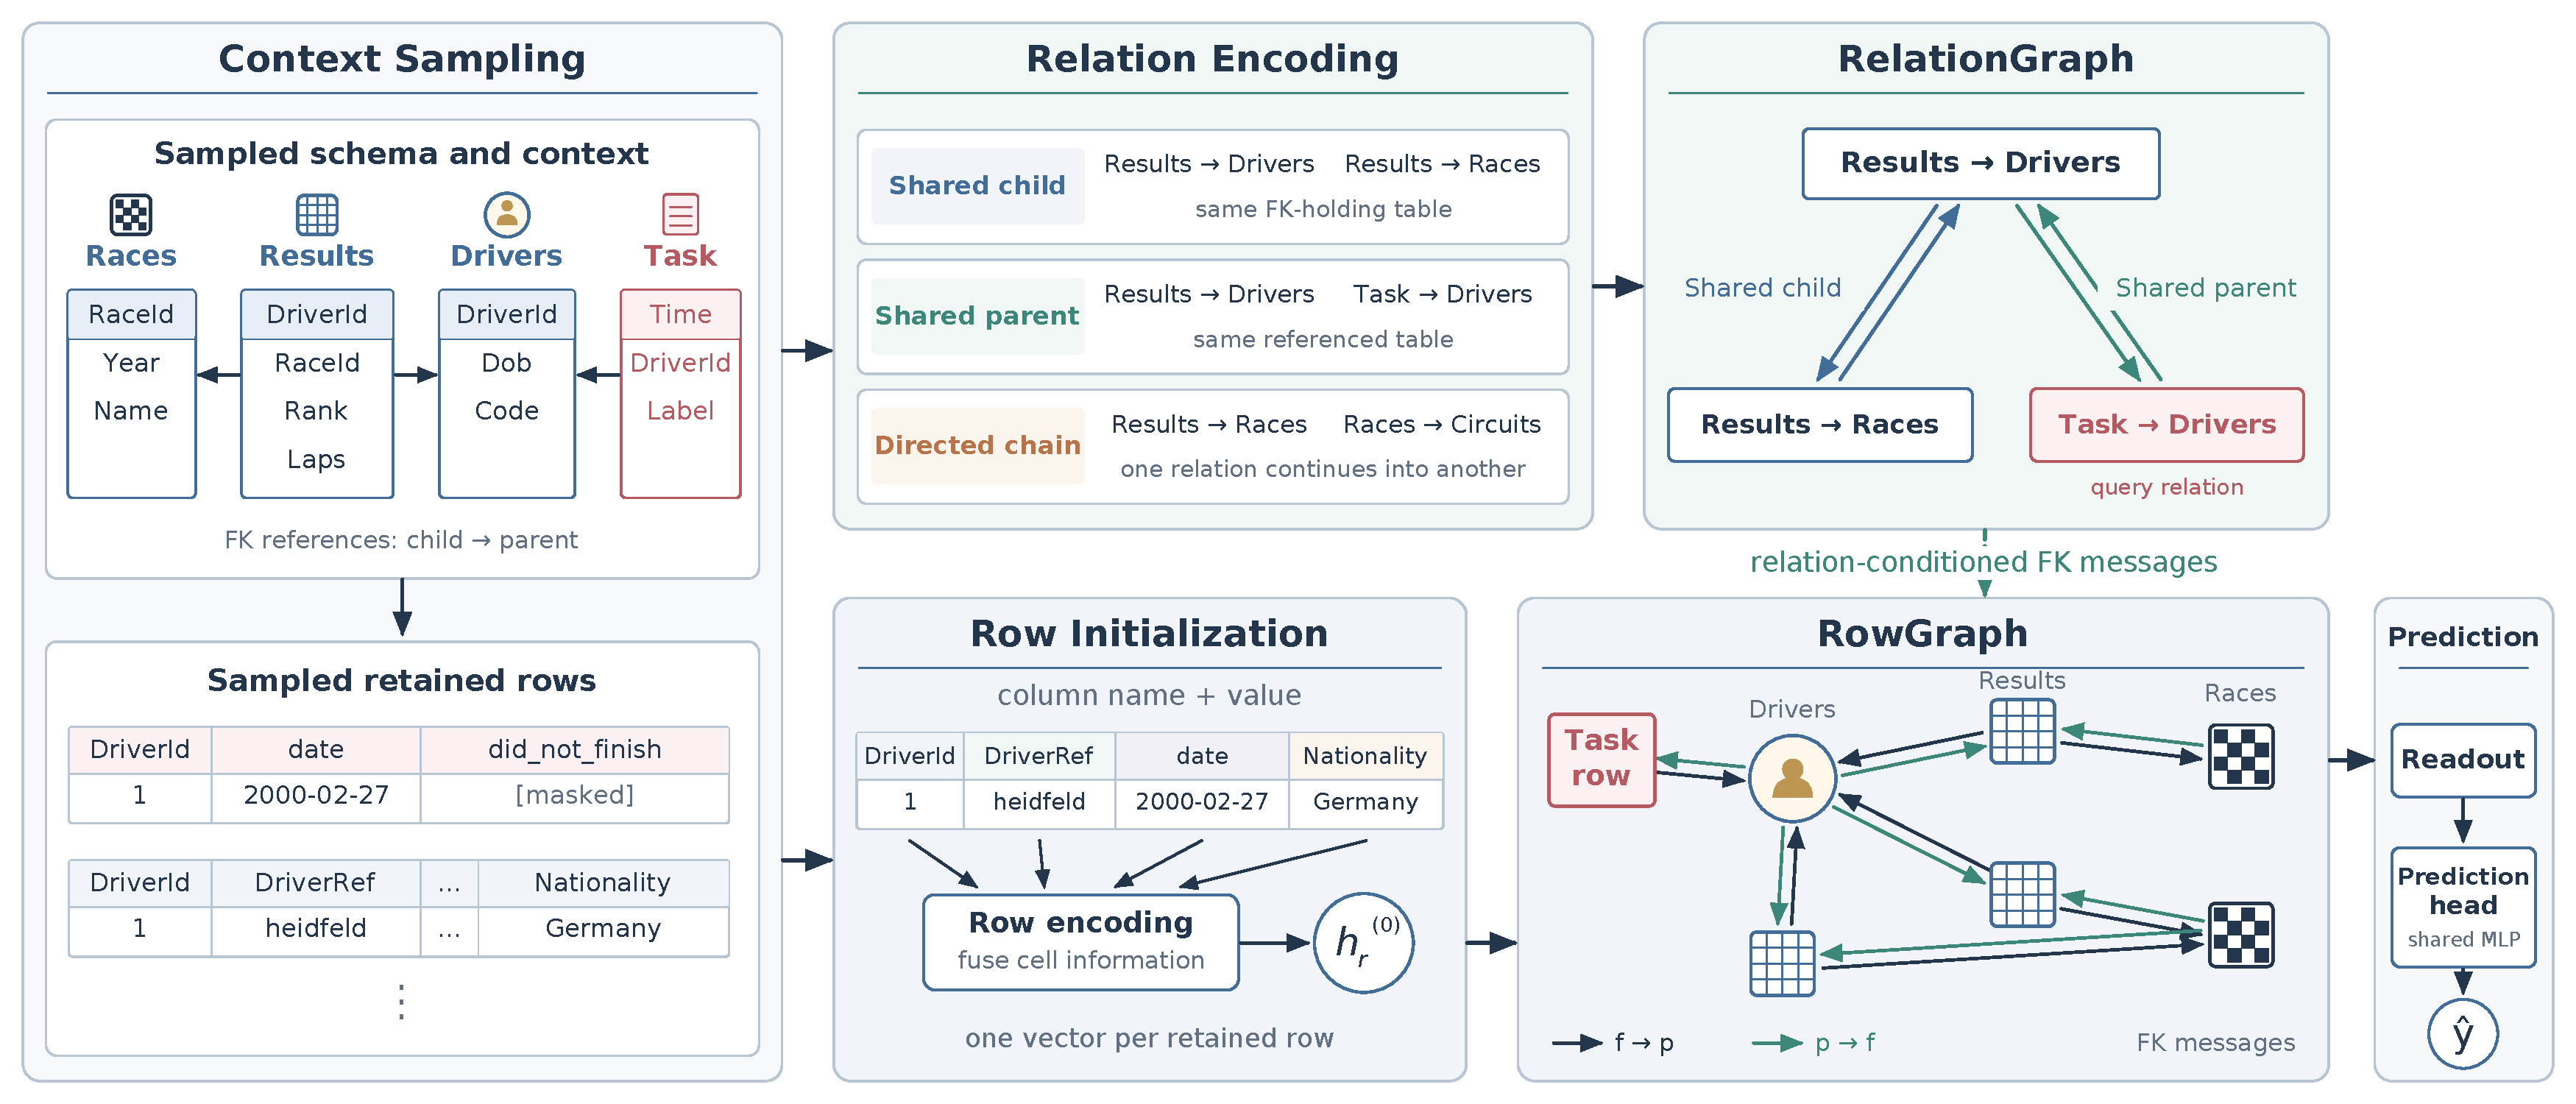
\includegraphics[width=\textwidth]{figures/architecture.pdf}
% %   \caption{High-level overview of \model{}.  A bounded temporal context is
% %   sampled, and visible heterogeneous cells are pooled once into row states.
% %   The retained PK--FK links instantiate two coupled graphs: an instance-level
% %   bidirectional row graph and a query-conditioned relation graph over ordered
% %   child--parent table pairs.  The relation states condition the corresponding
% %   foreign-to-primary ($\fkp$) and primary-to-foreign ($\pkf$) row messages,
% %   after which a shared candidate scorer, abstracted by the MLP block, produces
% %   the prediction.  Candidate nodes and label edges are omitted for clarity;
% %   red marks the query table, row, and seeded relation.}
% %   \label{fig:architecture}
% % \end{figure*}

% % We introduce \model{}, a compact row-level architecture for binary temporal entity classification on held-out relational databases (Figure~\ref{fig:architecture}).  Its context module samples a bounded, temporally valid neighborhood and aggregates visible heterogeneous cells into one representation per row.  Its relation-guidance module constructs a query-conditioned relation graph from the local PK--FK structure and uses shared structural interactions to infer relation representations without learned schema-specific identifiers.  Its row-reasoning module uses these representations to guide bidirectional message passing over the row graph, followed by a shared entity-classification readout.

% % Our contributions are:
% % \begin{itemize}
% %   \item We develop a compact row-graph architecture that combines bounded temporal context construction, heterogeneous row encoding, relation-guided message passing, and a shared entity-classification readout.
% %   \item We construct query-specific relation representations from schema-local structural interactions rather than learned table or relation identifiers, allowing the same operators to be applied to held-out database schemas.
% %   \item We evaluate \model{} on ten binary RelBench tasks under leave-database-out transfer.  It achieves 69.7 macro AUROC with 2.78M trainable parameters, and removing relation guidance reduces the score to 67.6.  A controlled target-history-masking evaluation further measures how strongly predictions depend on the query entity's previous labels.
% % \end{itemize}

% \section{Introduction}
% \label{sec:introduction}

% Relational databases support predictive decisions in commerce, finance,
% science, and online platforms. Evidence for these predictions is often
% distributed across interconnected tables, requiring models to combine
% information about an entity with its associated records. RelBench makes
% these problems accessible to systematic study by providing real-world
% relational databases, predictive tasks, and standardized temporal splits
% \citep{robinson2024relbench}. Relational Deep Learning (RDL) addresses such
% tasks by learning to aggregate information along primary--foreign key
% (PK--FK) connections, reducing the need for manually designed joins and
% feature aggregation \citep{fey2024rdl}. However, in the common task-specific
% supervised setting, a new database or prediction target requires another
% cycle of model training and validation. Reusing a unified model across
% databases would reduce this repeated effort and support prediction when
% target-task training resources are limited.

% Recent relational foundation models have demonstrated the feasibility of
% cross-database prediction \citep{ranjan2026rt}. A central design challenge is
% to preserve relation-specific computation while sharing parameters across
% different schemas. Consider Formula~1: both
% \texttt{Results}$\rightarrow$\texttt{Drivers} and
% \texttt{Results}$\rightarrow$\texttt{Races} are child-to-parent connections,
% but one associates a result with a driver, whereas the other places it
% within a race. Their shared direction alone does not capture these different
% roles in connecting predictive evidence. Representing relations beyond their
% FK direction allows the model to explicitly condition information
% propagation on the connections involved. Across databases, however, table
% identities and relation vocabularies change, making it necessary to construct
% such representations without relying on a fixed set of learned relation
% embeddings. Inspired by ULTRA \citep{galkin2024ultra}, we construct a
% query-conditioned RelationGraph whose nodes represent ordered child--parent
% table pairs. Shared operators encode their structural interactions to
% generate relation representations that can be applied to unseen schemas.

% \begin{figure*}[t]
%   \centering
%   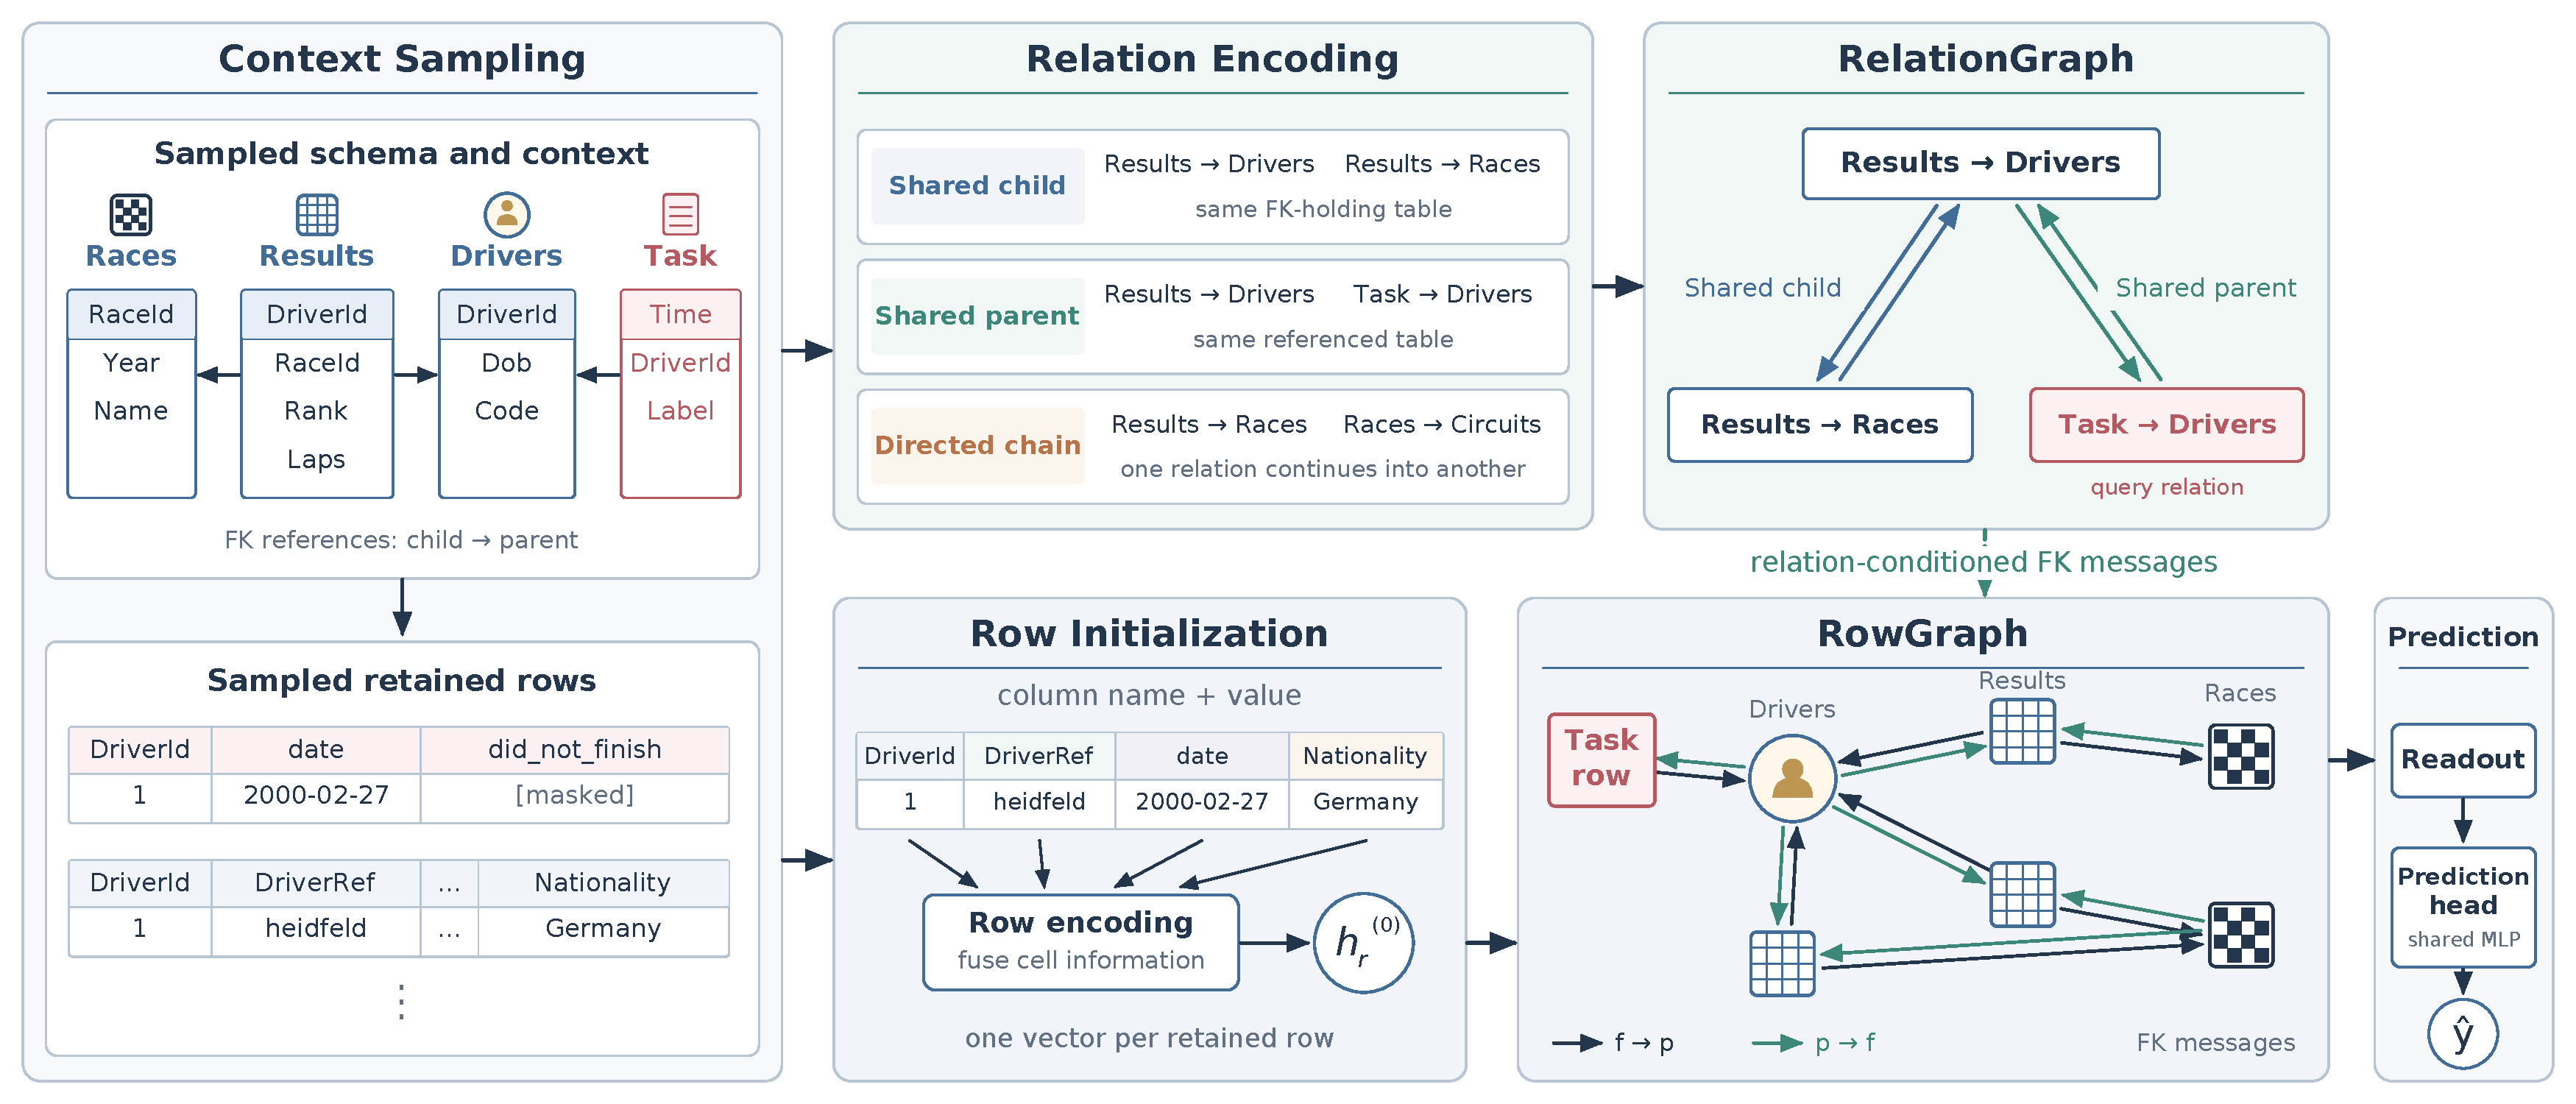
\includegraphics[width=\textwidth]{figures/architecture.pdf}
%   \caption{High-level overview of \model{}.  A bounded temporal context is
%   sampled, and visible heterogeneous cells are pooled once into row states.
%   The retained PK--FK links instantiate two coupled graphs: an instance-level
%   bidirectional row graph and a query-conditioned relation graph over ordered
%   child--parent table pairs.  The relation states condition the corresponding
%   foreign-to-primary ($\fkp$) and primary-to-foreign ($\pkf$) row messages,
%   after which a shared candidate scorer, abstracted by the MLP block, produces
%   the prediction.  Candidate nodes and label edges are omitted for clarity;
%   red marks the query table, row, and seeded relation.}
%   \label{fig:architecture}
% \end{figure*}

% These representations guide how information propagates between records;
% prediction further requires integrating record contents and task context.
% We therefore introduce \model{} (Figure~\ref{fig:architecture}), which
% couples RelationGraph with a row-level reasoning and candidate-prediction
% architecture. Within a bounded, temporally filtered context, shared encoders
% aggregate heterogeneous cell values into row representations, and retained
% PK--FK links connect these rows into a graph. The inferred relation
% representations condition bidirectional messages, guiding multi-hop
% aggregation of evidence across records. To incorporate historical task
% labels, we further augment the graph with two shared class-candidate nodes
% representing False and True. These nodes aggregate messages from context rows
% with matching labels, and a shared scorer compares the query row with each
% candidate to produce the prediction. Together, these components combine
% transferable relation representations, compact row-level reasoning, and
% context-aware prediction using parameters shared across databases and tasks.

% Our contributions are:
% \begin{itemize}
%   \item We introduce a query-conditioned RelationGraph to construct
%   transferable relation representations.
%   \item We combine relation-guided RowGraph reasoning with shared True/False
%   candidate nodes for prediction across databases.
%   \item We evaluate \model{} on ten binary RelBench tasks, comparing its
% accuracy and parameter efficiency with baselines, examining the effect of
% model size, and analyzing which information the trained model relies on.

% \end{itemize}


% \section{Introduction}
% \label{sec:introduction}

% Relational databases support predictive decisions in commerce, finance,
% science, and online platforms. The evidence for a prediction is usually
% spread over linked tables: whether a Formula~1 driver will fail to finish the
% next race depends on the driver's earlier results, the races in which they
% were obtained, and the other drivers in those races. Relational Deep Learning
% (RDL) represents rows as nodes and primary--foreign key (PK--FK) references as
% edges, and learns to aggregate this evidence with graph neural networks (GNNs)
% \citep{fey2024rdl}; RelBench provides real-world databases and temporal
% prediction tasks for this setting \citep{robinson2024relbench}. These models,
% however, are trained for one database and one task, so every new database or
% prediction target requires another cycle of training and validation.
% Cross-dataset entity classification removes this cycle: a model trained on a
% collection of databases predicts entity labels in an unseen database without
% updating its parameters.

% Relational foundation models have made this setting feasible
% \citep{ranjan2026rt,ranjan2026rtj,kothapalli2026plurel,hudovernik2026kumorfm2}.
% To cope with databases whose tables and columns differ, they represent a
% database as generic units, such as cells in \RT{} \citep{ranjan2026rt} or rows
% and sampled examples in KumoRFM-2 \citep{hudovernik2026kumorfm2}, and use
% attention to learn from data which of these units are relevant to a
% prediction; RDBLearn similarly relies on a tabular in-context learner that
% attends over thousands of labeled examples \citep{xu2026rdblearn}. Much of
% what this attention has to discover is, however, structural. \RT{}'s own
% analysis attributes its zero-shot transfer to task context, relational
% attention patterns, and schema semantics \citep{ranjan2026rt}; the first two
% amount to knowing which records carry labels and which records are linked.
% A database states this information explicitly: PK--FK references identify
% linked records, the schema specifies how tables are connected, and the task
% table and timestamps provide the label history and its temporal order.
% Learning it through attention costs model capacity and computation; \RT{},
% for example, uses 22M parameters and attends over cell-level tokens in every
% layer.

% GNNs take the opposite approach. Their aggregation follows PK--FK edges
% directly, which makes them compact, but they distinguish structure through
% parameters tied to one schema: an encoder for each table, a weight matrix for
% each relation, and an output head for each task
% \citep{fey2024rdl,chen2025relgnn}. These parameters make structural
% distinctions explicit. In Formula~1, \texttt{Results}$\rightarrow$\texttt{Drivers}
% and \texttt{Results}$\rightarrow$\texttt{Races} are both child-to-parent links,
% but the first connects a result to the driver who obtained it and the second
% to the race in which it occurred; a relation-specific weight lets the model
% treat the two kinds of evidence differently. In an unseen database none of
% these parameters is defined. Griffin shares its encoders across databases, but
% aggregates cells with attention and is fine-tuned for each downstream task
% \citep{wang2025griffin}. Simply removing relation-specific weights makes a GNN
% transferable but discards the distinctions they encode, since messages along
% all PK--FK links are then processed alike. On F1 driver-DNF, for instance,
% retraining our model without its relation representations lowers AUROC from
% 81.2 to 74.2 (Section~\ref{sec:result}).
% % TODO: add the retrained ablation (results/ablation/retrained) to Section 5;
% % the numbers above are seed 2 and predate the relation-key fix.

% The central challenge is therefore to retain the efficiency of
% structure-following aggregation while expressing these structural distinctions
% without parameters specific to any database. Meeting it makes prediction on an
% unseen database direct, because the database structure rather than learned
% attention specifies which records are related and how, and efficient, because
% no capacity is spent on recovering this structure from data.

% \begin{figure*}[t]
%   \centering
%   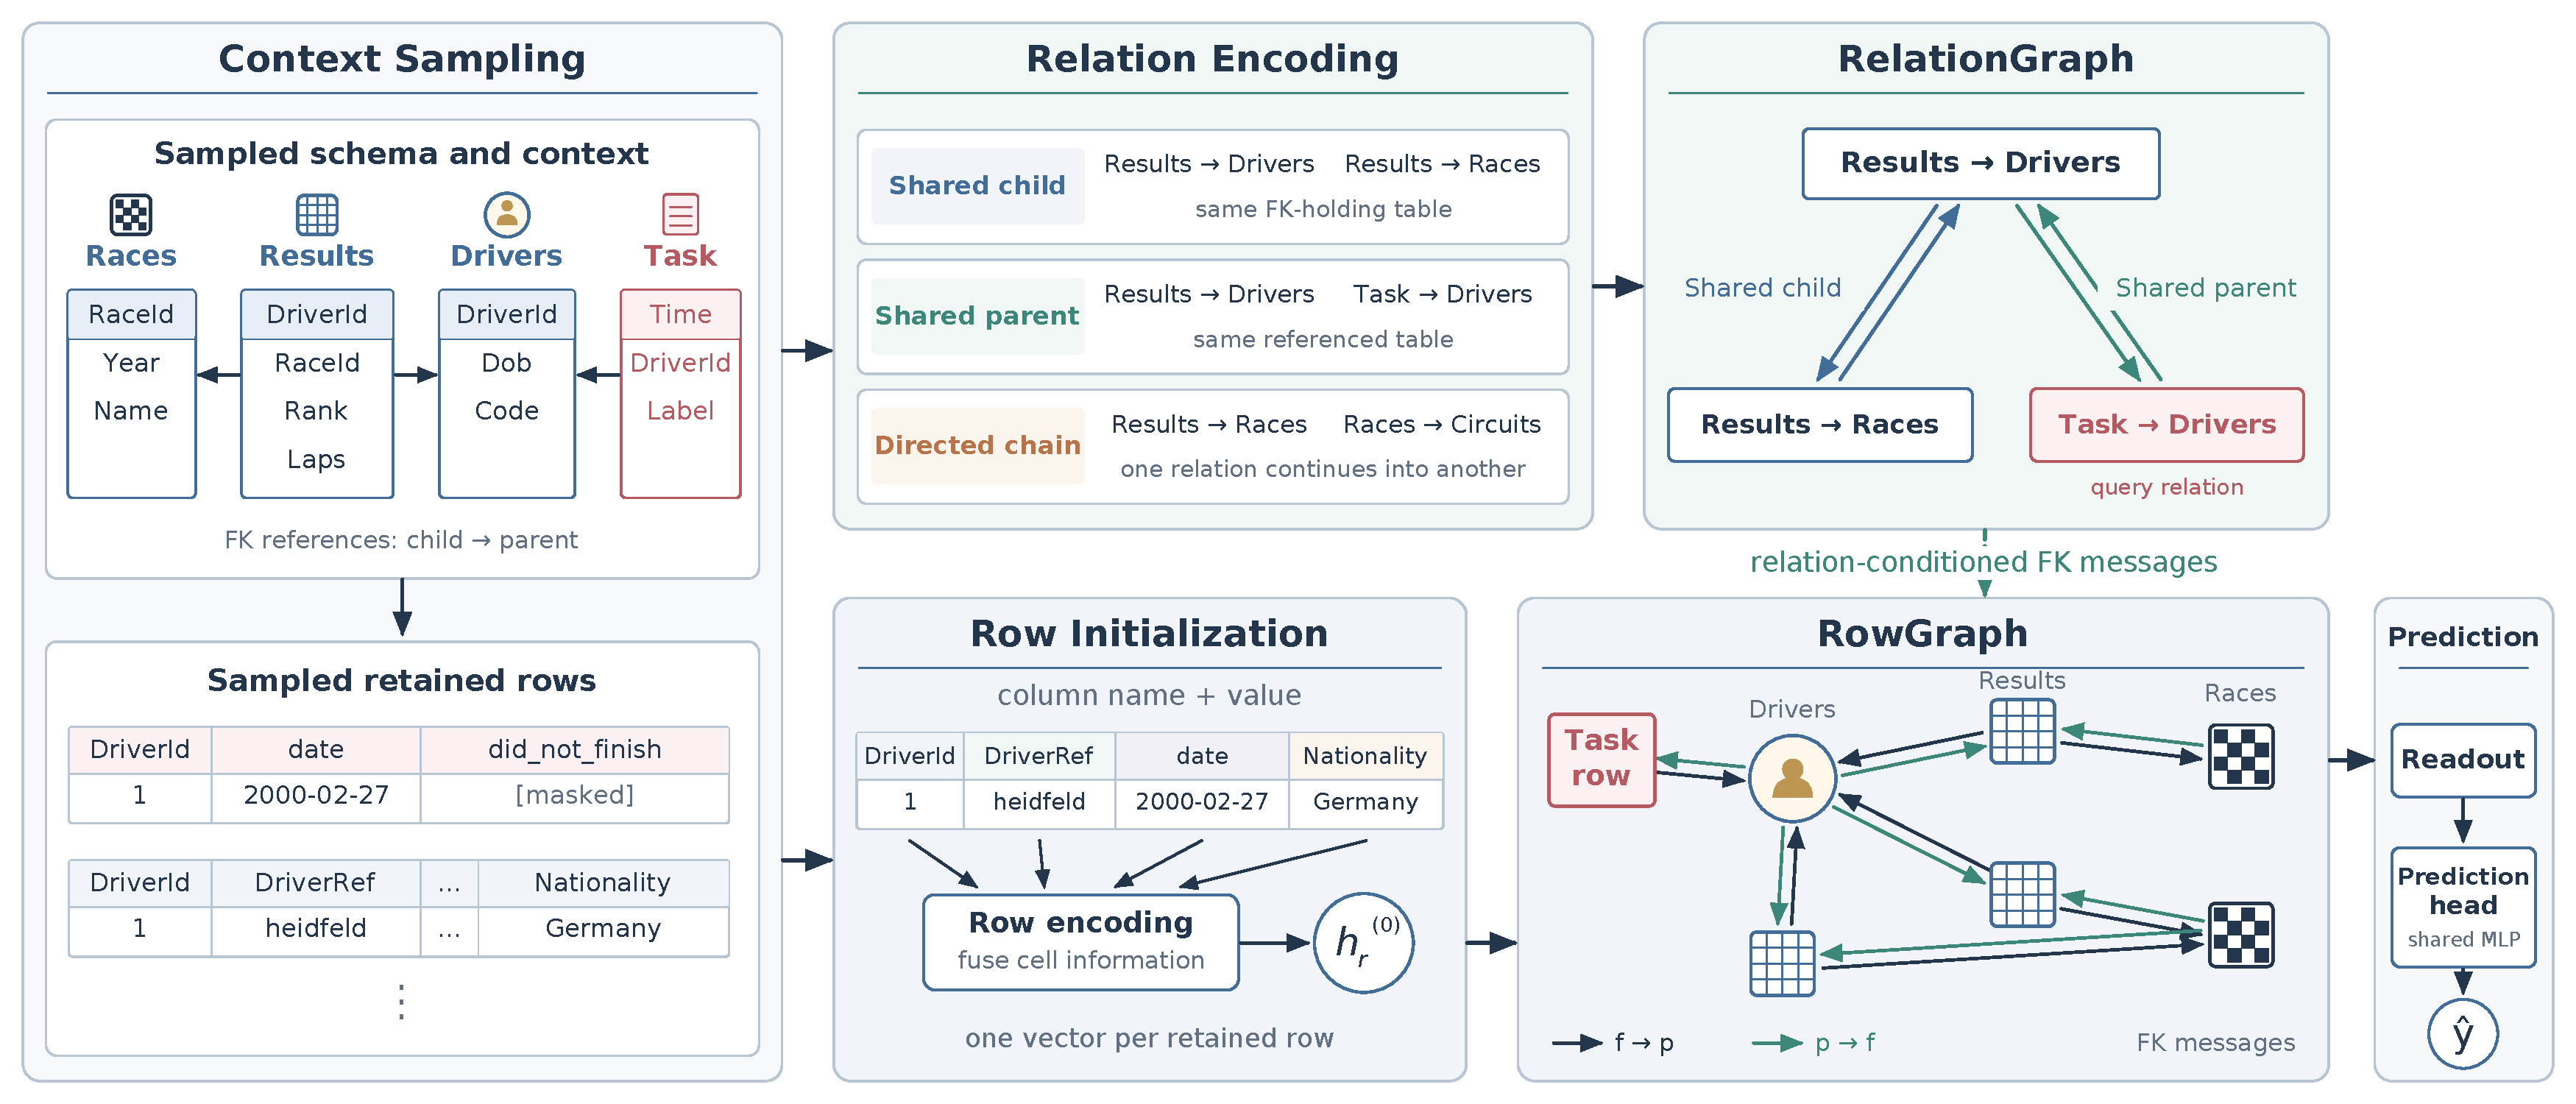
\includegraphics[width=\textwidth]{figures/architecture.pdf}
%   \caption{High-level overview of \model{}.  A bounded temporal context is
%   sampled, and visible heterogeneous cells are pooled once into row states.
%   The retained PK--FK links instantiate two coupled graphs: an instance-level
%   bidirectional row graph and a query-conditioned relation graph over ordered
%   child--parent table pairs.  The relation states condition the corresponding
%   foreign-to-primary ($\fkp$) and primary-to-foreign ($\pkf$) row messages,
%   after which a shared candidate scorer, abstracted by the MLP block, produces
%   the prediction.  Candidate nodes and label edges are omitted for clarity;
%   red marks the query table, row, and seeded relation.}
%   \label{fig:architecture}
% \end{figure*}

% We address this challenge with \model{} (Figure~\ref{fig:architecture}), a
% lightweight GNN whose parameters are tied only to roles that every database
% shares. Each distinction above can be derived from structure present in any
% database. \emph{Linked records} follow from PK--FK references: as in \RT{},
% cells are encoded from their values and column names with encoders shared
% across tables; \model{} pools them once into one vector per record and passes
% messages along PK--FK links with two edge types, child-to-parent and
% parent-to-child, that are common to all databases. \emph{The role of a
% relation} follows from how it shares tables with other relations: adapting
% the relation graph of knowledge-graph foundation models
% \citep{lee2023ingram,galkin2024ultra}, \model{} treats each child--parent
% table pair as a relation, connects relations that share a table, and
% propagates from the relation of the query to derive representations that
% condition the messages along each relation. \emph{Labels} follow from the
% task table: records with known labels are connected to one node per class,
% and the query is scored against these nodes, so no task-specific output layer
% is needed; each timestamped record also carries its time relative to the
% prediction. Because the database structure, rather than learned attention,
% determines how information is aggregated, all computation after cell encoding
% scales with the number of records and links rather than cells.

% On ten binary classification tasks from RelBench under leave-database-out
% transfer, \model{} reaches \mainAUROC{} macro AUROC with \mainParams{}
% parameters, on par with the strongest baseline, which uses about eight times as
% many parameters, and its accuracy grows with width to \wideAUROC{} at
% \wideParams{} parameters (Section~\ref{sec:standard_results}). Our analysis
% shows that two-hop neighborhoods suffice and that the entity's own label
% history is the dominant signal (Section~\ref{sec:case_study}).

% Our contributions are:
% \begin{itemize}
%   \item We identify the schema-specific parameters through which relational
%   GNNs encode structure and propose \model{}, a row-level GNN that replaces
%   them with counterparts shared across databases, so that the database
%   structure, rather than learned attention, determines how information is
%   aggregated.
%   \item We adapt the relation graph of knowledge-graph foundation models to
%   relational databases, defining relations as child--parent table pairs and
%   using the resulting representations to condition message passing between
%   records, so that relations in unseen schemas are distinguished without
%   relation-specific parameters.
%   \item We evaluate \model{} on ten RelBench tasks under leave-database-out
%   transfer, showing that with \mainParams{} parameters it performs on par with
%   or better than attention-based baselines about eight times its size, and
%   analyze which information it relies on.
% \end{itemize}

\section{Introduction}
\label{sec:introduction}

Relational databases support predictive decisions in commerce, finance,
science, and online platforms. The evidence for a prediction is usually
spread over linked tables: whether a Formula~1 driver will fail to finish the
next race depends on the driver's earlier results, the races in which they
were obtained, and the other drivers in those races. Relational Deep Learning
(RDL) represents rows as nodes and primary--foreign key (PK--FK) references as
edges, and learns to aggregate this evidence with graph neural networks (GNNs)
\citep{fey2024rdl}; RelBench provides real-world databases and temporal
prediction tasks for this setting \citep{robinson2024relbench}. These models,
however, are trained for one database and one task, so every new database or
prediction target requires another cycle of training and validation.
Cross-dataset entity classification removes this cycle: a model trained on a
collection of databases predicts entity labels in an unseen database without
updating its parameters.

Relational foundation models have made this setting feasible
\citep{ranjan2026rt,ranjan2026rtj,kothapalli2026plurel,hudovernik2026kumorfm2}.
To cope with databases whose tables and columns differ, they represent a
database as generic units, such as cells in \RT{} \citep{ranjan2026rt} or rows
and sampled examples in KumoRFM-2 \citep{hudovernik2026kumorfm2}, and use
attention to learn from data which of these units are relevant to a
prediction; RDBLearn similarly relies on a tabular in-context learner that
attends over thousands of labeled examples \citep{xu2026rdblearn}. Much of
what this attention has to discover is, however, structural. \RT{}'s own
analysis attributes its zero-shot transfer to task context, relational
attention patterns, and schema semantics \citep{ranjan2026rt}; the first two
amount to knowing which records carry labels and which records are linked.
A database states this information explicitly: PK--FK references identify
linked records, the schema specifies how tables are connected, and the task
table and timestamps provide the label history and its temporal order.
Learning it through attention costs model capacity and computation; \RT{},
for example, uses 22M parameters and attends over cell-level tokens in every
layer.

GNNs take the opposite approach. Their aggregation follows PK--FK edges
directly, which makes them compact, but they distinguish structure through
parameters tied to one schema: an encoder for each table, a weight matrix for
each relation, and an output head for each task
\citep{fey2024rdl,chen2025relgnn}. These parameters make structural
distinctions explicit. In Formula~1, \texttt{Results}$\rightarrow$\texttt{Drivers}
and \texttt{Results}$\rightarrow$\texttt{Races} are both child-to-parent links,
but the first connects a result to the driver who obtained it and the second
to the race in which it occurred; a relation-specific weight lets the model
treat the two kinds of evidence differently. In an unseen database none of
these parameters is defined. Griffin shares its encoders across databases, but
aggregates cells with attention and is fine-tuned for each downstream task
\citep{wang2025griffin}. Simply removing relation-specific weights makes a GNN
transferable, but it then applies the same transformation to messages along
every PK--FK link, so the distinction has to be recovered from record content,
as attention-based models do from the table and column names attached to each
token \citep{ranjan2026rt}.
On F1 driver-DNF, for instance,
% retraining our model without its relation representations lowers AUROC from
% 81.2 to 74.2 (Section~\ref{sec:result}).

The central challenge is therefore to retain the efficiency of
structure-following aggregation while expressing these structural distinctions
without parameters specific to any database. Meeting it makes prediction on an
unseen database direct, because the database structure rather than learned
attention specifies which records are related and how, and efficient, because
no capacity is spent on recovering this structure from data.

\begin{figure*}[t]
  \centering
  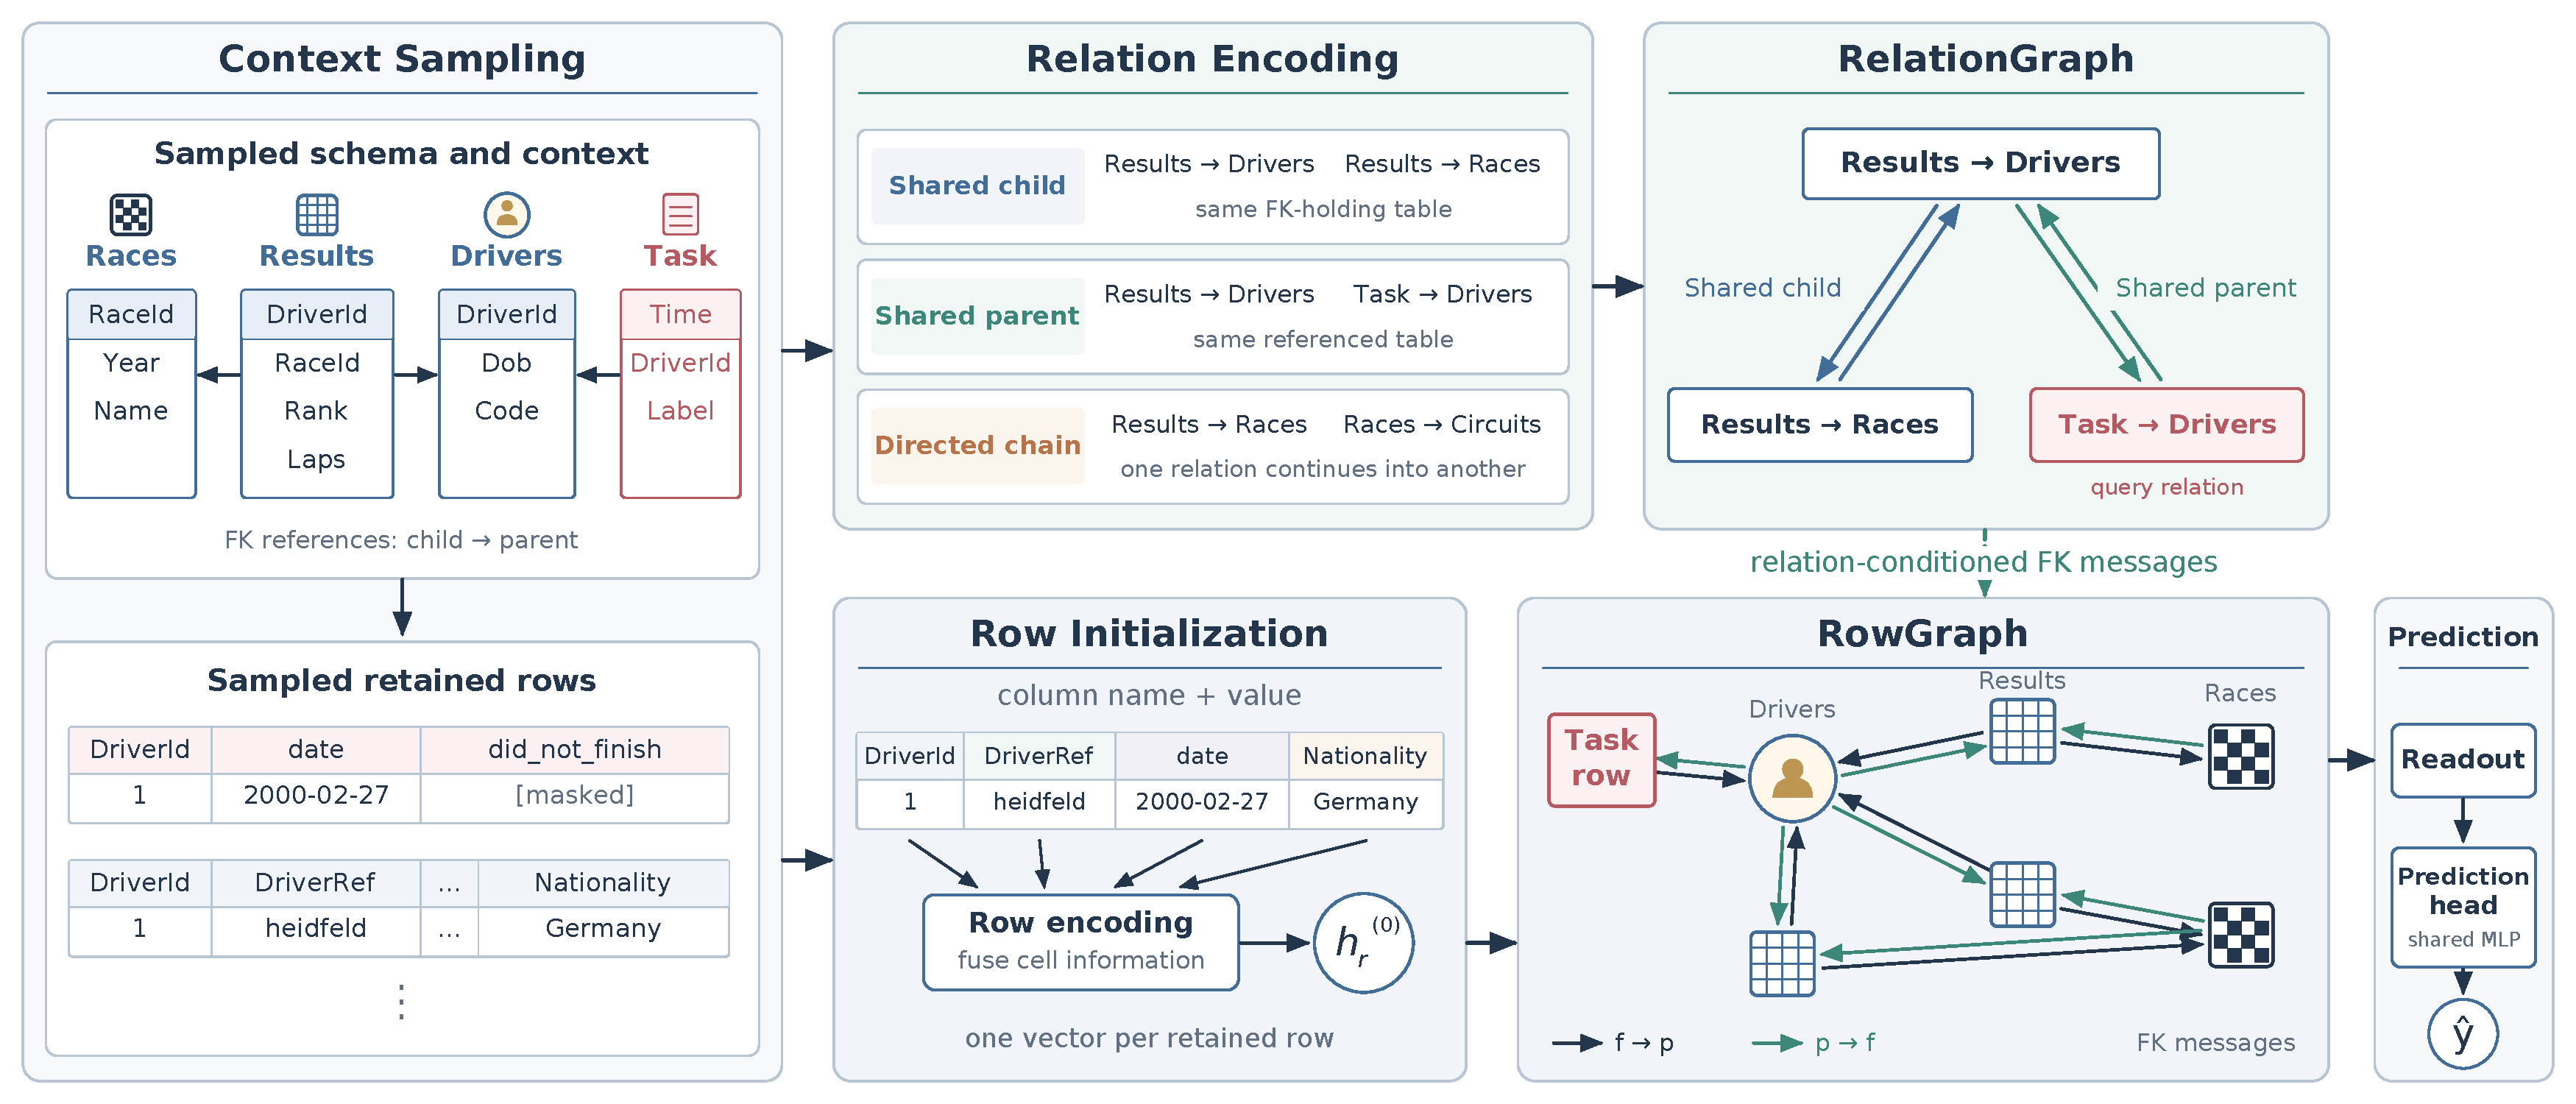
\includegraphics[width=\textwidth]{figures/architecture.pdf}
  \caption{Overview of \model{}. Context Sampling collects a bounded context
  around the query row that respects the prediction time: the tables and
  foreign-key references it contains (upper panel) and the sampled rows
  (lower panel). Row Initialization encodes the cells of each row into one
  vector. Relation Encoding links the foreign-key relations that share a
  table, and RelationGraph computes one representation per relation,
  conditioned on the query relation. These representations condition the
  child-to-parent (f$\rightarrow$p) and parent-to-child (p$\rightarrow$f)
  messages of RowGraph. Prediction compares the final state of the query row
  with class nodes that collect the labels of earlier task rows; the class
  nodes and their edges are omitted from the drawing. Red marks the query
  table, the query row, and the query relation.}
  \label{fig:architecture}
\end{figure*}

We address this challenge with \model{} (Figure~\ref{fig:architecture}), a
lightweight GNN whose parameters are tied only to roles that every database
shares. Each distinction above can be derived from structure present in any
database. \emph{Linked records} follow from PK--FK references: as in \RT{},
cells are encoded from their values and column names with encoders shared
across tables; \model{} pools them once into one vector per record and passes
messages along PK--FK links with two edge types, child-to-parent and
parent-to-child, that are common to all databases. \emph{The role of a
relation} follows from how it shares tables with other relations: adapting
the relation graphs that knowledge-graph models use to represent unseen
relations \citep{lee2023ingram,galkin2024ultra}, \model{} treats each child--parent
table pair as a relation, connects relations that share a table, and
propagates from the relation of the query to derive representations that
condition the messages along each relation. \emph{Labels} follow from the
task table: records with known labels are connected to one node per class,
and the query is scored against these nodes, so no task-specific output layer
is needed; each timestamped record also carries its time relative to the
prediction. Because the database structure, rather than learned attention,
determines how information is aggregated, all computation after cell encoding
scales with the number of records and links rather than cells.

On ten binary classification tasks from RelBench under leave-database-out
transfer, \model{} reaches \mainAUROC{} macro AUROC with \mainParams{}
parameters, on par with the strongest baseline, which uses about eight times as
many parameters, and its accuracy grows with width to \wideAUROC{} at
\wideParams{} parameters (Section~\ref{sec:standard_results}). Our analysis
shows that two-hop neighborhoods suffice and that the entity's own label
history is the dominant signal (Section~\ref{sec:case_study}).

Our contributions are:
\begin{itemize}
  \item We identify the schema-specific parameters through which relational
  GNNs encode structure and propose \model{}, a row-level GNN that replaces
  them with counterparts shared across databases, so that the database
  structure, rather than learned attention, determines how information is
  aggregated.
  \item We bring to relational databases the relation graphs that
  knowledge-graph models use to represent unseen relations, defining relations
  as child--parent table pairs and
  using the resulting representations to condition message passing between
  records, so that relations in unseen schemas are distinguished without
  relation-specific parameters.
  \item We evaluate \model{} on ten RelBench tasks under leave-database-out
  transfer, showing that with \mainParams{} parameters it performs on par with
  or better than attention-based baselines about eight times its size, and
  analyze which information it relies on.
\end{itemize}
\section{Related Work}
\label{sec:related}

\subsection{Graph Neural Networks on Relational Databases}
RDL represents a relational database as a heterogeneous temporal graph with
one node per row and one edge per PK--FK reference, and learns to aggregate
information across tables with GNNs \citep{fey2024rdl}; RelBench
standardizes databases, temporal prediction tasks, and evaluation splits for
this setting \citep{robinson2024relbench}. RelGNN introduces atomic routes
and composite message passing to handle many-to-many relationships
\citep{chen2025relgnn}, and RelGT tokenizes each node into features, type,
hop distance, time, and local structure for a graph transformer
\citep{dwivedi2026relgt}. In RDL and RelGNN, messages flow only along PK--FK
references, so the database structure rather than learned attention decides
which rows interact. These models, however, encode the structure through
parameters tied to one schema: column encoders for each table, node and edge
types defined by the schema, separate weights for each relation or atomic
route, and an output head for each task
\citep{fey2024rdl,robinson2024relbench,chen2025relgnn}. They are therefore
trained anew for every database and task. \model{} keeps their
structure-following aggregation but replaces these schema-specific parameters
with counterparts shared across databases.

\subsection{Relational Foundation Models}
Relational foundation models reuse one pretrained model across databases.
Griffin pretrains shared encoders and decoders with relational message
passing, gathering the cells of each row through cross-attention over column
names, and is fine-tuned on each downstream task \citep{wang2025griffin}.
\RT{} removes fine-tuning: each cell is a token that carries an embedding of
its column and table names, the task is specified through the task table,
and relational attention over columns, rows, and PK--FK links lets the model
predict on unseen databases without updating its parameters
\citep{ranjan2026rt}. Later work improves pretraining and context: PluRel
synthesizes relational databases for pretraining
\citep{kothapalli2026plurel}, RT-J scales up pretraining for few-shot
prediction \citep{ranjan2026rtj}, and OpenRFM adds a batch-level in-context
learning layer to cope with sparse label coverage in sampled neighborhoods
\citep{chen2026openrfm}. KumoRFM-2 attends along the row, column, foreign-key,
and cross-sample dimensions \citep{hudovernik2026kumorfm2}. In \RT{}, Griffin,
and KumoRFM-2, attention over cells, rows, or examples determines which parts
of the relational context inform a prediction, and \RT{} keeps cell-level
tokens in every layer with about 22M parameters. \model{} instead lets the
database structure decide which records exchange information and learns only
how the exchanged messages are transformed, so it needs no attention and has
\mainParams{} parameters at its default width; it pools the
cells of each record once, giving up cell-level detail in exchange for
computation that scales with records rather than cells.

A second family flattens each entity's neighborhood into aggregate features
fixed in advance by deep feature synthesis and passes them to a tabular
in-context learner \citep{xu2026rdblearn,wang2026rdbpfn}. Their relational
encoding is therefore fixed rather than learned, and, like KumoRFM-2, they
rely on a support set of labeled
examples from the target task, whereas \RT{} and \model{} read only the
labels in the sampled context of each prediction; we follow the protocol of
\RT{}.
% Moved out of this paragraph (for an experiments-section comparison, if any):
% RDB-PFN reads 64-1,024 labeled examples and excludes the target entity's own
% label history; on our ten tasks its macro AUROC is 65.3 with 64 and 72.0 with
% 1,024 (wang2026rdbpfn Tables 6 and 10). RDBLearn reads up to 10,000.

\subsection{Transferable Relation Representations}
Knowledge graphs pose a related transfer problem, because the relation
vocabulary changes between training and inference graphs. InGram builds a
graph over relations whose edge weights reflect how many entities two
relations share, and derives embeddings of unseen relations from it
\citep{lee2023ingram}. ULTRA connects relations through four interactions
(head--head, tail--tail, head--tail, and tail--head), conditions the relation
representations on the query relation, and uses them for link prediction,
which enables zero-shot transfer across knowledge graphs
\citep{galkin2024ultra}. \model{} adapts this construction to relational
databases: a relation is a child--parent table pair, two relations are
adjacent when they share a table, and the resulting representations
condition message passing between records that carry their own content, for
entity classification rather than link prediction.

% ---- Previous version (before the 2026-11-02 rewrite), kept for reference ----
% \section{Related Work}
% \label{sec:related}
%
% \subsection{Relational Deep Learning}
% RDL turns a relational database into a graph of rows connected by PK--FK references and learns to aggregate information across tables \citep{fey2024rdl}.  RelBench standardizes databases, temporal prediction tasks, and evaluation splits for this setting \citep{robinson2024relbench}.  RelGNN uses atomic routes and composite message passing to better capture the structure of database graphs, including many-to-many relationships \citep{chen2025relgnn}. RelGT combines row features with type, hop, time, and local-structure information in a graph transformer \citep{dwivedi2026relgt}.  These approaches establish the value of explicitly modeling how rows are connected and how information passes between them. These models are typically trained for a specific database and prediction task, so applying them to a new database generally requires further training. Our work retains their row-graph representation and PK--FK message passing, but focuses on transfer to unseen databases without updating model parameters.
%
% \subsection{Foundation Models for Relational Data}
% Foundation models approach relational prediction through reusable representations and pretraining. This line includes both relational database foundation models and knowledge-graph foundation models; they share a transfer goal but differ in their inputs and prediction tasks.
%
% \subsection{Relational Database Foundation Models}
% Griffin combines shared encoders and decoders with relational message passing,
% but its downstream evaluation still requires task-specific fine-tuning
% \citep{wang2025griffin}. The Relational Transformer (\RT{}) removes this requirement by using task-table
% context and relational attention to predict on unseen databases without
% updating parameters \citep{ranjan2026rt}. Subsequent work addresses limitations
% in pretraining data and contextual labels. PluRel tackles the scarcity of
% diverse databases through synthetic relational data generation
% \citep{kothapalli2026plurel}. OpenRFM identifies sparse label coverage in
% \RT{}'s sampled neighborhoods and adds batch-level in-context learning
% \citep{chen2026openrfm}. RT-J improves few-shot prediction by scaling
% pretraining and revising context retrieval and training objectives
% \citep{ranjan2026rtj}.
%
% Alongside these improvements to pretraining and context, the granularity of
% relational computation remains a design choice. \RT{} maintains cell-level
% representations throughout its backbone. RDBLearn highlights the risk of
% losing task-relevant information through cross-column compression and
% instead preserves columns for a tabular in-context learner
% \citep{xu2026rdblearn}. We investigate whether pooling cells into compact row
% representations can still support competitive transfer when combined with
% explicit relation guidance. \model{} uses RelationGraph to guide RowGraph
% message passing and shared class-candidate nodes to aggregate labeled context
% for prediction.
% Griffin connects graph-centric RDL with foundation-model pretraining through shared encoders, relational message passing, and unified decoding \citep{wang2025griffin}.  It is an early point of contact between the two lines, with downstream transfer based on task adaptation.  \RT{} takes a frozen-transfer approach through task-table prompting, cell tokenization, and attention over columns, rows, and PK--FK neighborhoods \citep{ranjan2026rt}.  It is our closest comparator under the ten-task leave-database-out suite.
%
% Subsequent work explores several ways to improve reuse.  PluRel generates diverse synthetic schemas, PK--FK connectivity, and features for pretraining \citep{kothapalli2026plurel}.  RDBLearn combines a column-preserving relational encoder with a tabular in-context learner \citep{xu2026rdblearn}, while KumoRFM-2 combines row, column, FK, and cross-sample processing \citep{hudovernik2026kumorfm2}.  OpenRFM studies sparse contextual label coverage and introduces a batch-level support channel \citep{chen2026openrfm}; These methods demonstrate that relational foundation models encompass several representation choices. Our work investigates how relation-specific computation can be shared across database schemas, using structurally inferred relation states to guide prediction over compact row representations. We evaluate this design under the leave-database-out protocol used by \RT{}.
%
% \paragraph{Knowledge-graph foundation models.}
% Knowledge graphs expose a related transfer problem: entity and relation vocabularies can change between training and inference. Inductive methods such as InGram construct relation graphs to represent previously unseen relations \citep{lee2023ingram}.  Building on the goal of reusable graph reasoning, ULTRA is a knowledge-graph foundation model that constructs query-conditioned relation states through four endpoint interactions: head--head, tail--tail, head--tail, and tail--head.  These states condition entity-level link prediction and allow a pretrained model to transfer across graphs with different vocabularies \citep{galkin2024ultra}. This principle provides the foundation-model side of our relation encoder. Its application to databases requires heterogeneous cell encoding, time-respecting context construction, and an entity-classification readout in addition to structural reasoning.
%
% \paragraph{Connecting the two lines.}
% \model{} combines RDL's row-level representation with the transferable relation-construction principle of knowledge-graph foundation models and is evaluated against representative relational foundation models. We instantiate a relation node for each retained ordered child--parent table pair, initialize the relations instantiated by the query row's outgoing FKs, and use their inferred states to condition both directions of FK message passing. The relation identities are local to the input database, while the encoders, interaction operators, and readout are shared. The resulting model tests whether this combination can support competitive frozen transfer with a small row-graph backbone. As in relational in-context learning, frozen weights can still use historical labels supplied in the input; we therefore evaluate both Standard context and a controlled intervention on the query entity's target history.

\section{Task Formulation}
\label{sec:task}

\paragraph{Relational database graph.}
Let $\mathcal V_D$ be the finite set of rows in a database $D$ and $\mathcal R_D$ its set of foreign-key columns. We represent $D$ as an attributed graph $\mathcal G_D=(\mathcal V_D,\mathcal R_D,\mathcal E_D,\mathcal A_D)$, where $\mathcal E_D\subseteq\mathcal V_D\times\mathcal R_D\times\mathcal V_D$. An edge $(r_c,\kappa,r_p)$ means that the foreign-key column $\kappa\in\mathcal R_D$ of child row $r_c$ references parent row $r_p$.  Different foreign-key columns may connect the same rows.  Each row $r$ belongs to a table $T_r$; $\mathcal A_D$ records its named cell values, semantic types, and timestamp $t_r$ when available.

\paragraph{Temporal entity classification.}
This paper focuses on entity classification, and our baseline comparisons
are restricted to this task type. A query $g=(r_g^\star,c_g^\star,t_g)$ specifies a query row, a target column, and a prediction time. The task is to predict the unknown binary target $y_g\in\{0,1\}$ associated with this query. The input consists of $g$ and a bounded, time-filtered context $\mathcal X_g$ sampled from $\mathcal G_D$, containing visible row attributes and PK--FK links. The label of the query row is masked (Section~\ref{sec:method:sampling}). The output is a probability $p_g$ and its corresponding class prediction:
\begin{equation}
 p_g=p_\theta(y_g=1\mid\mathcal X_g,g),
 \qquad \widehat y_g=\ind[p_g\geq\tfrac12].
 \label{eq:task}
\end{equation}

% \paragraph{Cross-database inference.}
% Given source databases $\mathcal D_{\mathrm{src}}$ and a target database
% $D^\star\notin\mathcal D_{\mathrm{src}}$, model parameters are optimized
% using only source-database training examples and remain fixed at inference.
% Representations are constructed from the target schema and query context,
% allowing inference on rows and relation types unseen during training.
% Following the benchmark protocol, temporally available labels in historical
% task rows may be included in the input context, but no target-database
% labels contribute to gradient-based parameter updates.
% We refer to this setting as \emph{frozen leave-database-out transfer},
% with target-validation-based checkpoint selection detailed in
% Section~\ref{sec:setup}.


\paragraph{Cross-database inference.}
Given source databases $\mathcal D_{\mathrm{src}}$ and a target database
$D^\star\notin\mathcal D_{\mathrm{src}}$, the goal is to apply a predictor
$p_\theta$ learned on $\mathcal D_{\mathrm{src}}$ to queries in $D^\star$
without updating $\theta$:
\begin{equation}
 \underbrace{p_\theta\!\left(y_g=1\mid\mathcal X_g,g\right)}
 _{D\in\mathcal D_{\mathrm{src}}}
 \quad\xrightarrow{\theta\ \text{fixed}}\quad
 \underbrace{p_\theta\!\left(y_g=1\mid\mathcal X_g^\star,g\right)}
 _{\text{inference on }D^\star},
 \label{eq:cross_database_transfer}
\end{equation}
where $\mathcal X_g$ and $\mathcal X_g^\star$ denote query contexts sampled
from $\mathcal G_D$ and $\mathcal G_{D^\star}$, respectively.
Representations are constructed from
the schema and query context of $D^\star$, allowing inference on rows and
relation types unseen during training.
Following the benchmark protocol, temporally available labels in historical
task rows may be included in $\mathcal X_g^\star$, but labels from $D^\star$
do not contribute to gradient-based parameter updates.
We refer to this setting as \emph{frozen leave-database-out transfer},
with target-validation-based checkpoint selection detailed in
Section~\ref{sec:setup}.
\section{Methodology}
\label{sec:method}

\model{} predicts the label $y_g$ of a query $g$ from its sampled context
$\mathcal X_g$ with parameters shared across databases. Following
Section~\ref{sec:introduction}, each block of Figure~\ref{fig:architecture}
uses one kind of structure that every database provides, in place of a
component that a relational GNN ties to one schema. Context Sampling gathers
the rows linked to the query (Section~\ref{sec:method:sampling}). Row
Initialization encodes each row from its cells and column names instead of a
per-table encoder (Section~\ref{sec:method:initialization}). RowGraph passes
messages along PK--FK references with edge types shared by all databases
instead of a weight matrix per relation (Section~\ref{sec:method:rowgraph}).
Relation Encoding and RelationGraph derive a representation of each relation
from the schema instead of a learned relation embedding
(Section~\ref{sec:method:relations}). Prediction compares the query with the
labeled rows of the task table instead of applying a task-specific output
head (Section~\ref{sec:method:prediction}). We use \emph{row} for a record of
a table, write $T_r$ and $t_r$ for the table and timestamp of row $r$, and
drop the query index $g$ when a quantity concerns a single query.

\subsection{Context Sampling}
\label{sec:method:sampling}

Following \RT{}, a prediction task is given as a task table whose rows hold a
foreign key to an entity, a timestamp, and a label. The query row
$r_g^\star$ is the task-table row whose label $y_g$ is to be predicted, and
its timestamp is the prediction time $t_g$. Context Sampling collects a
bounded input around $r_g^\star$ with the sampler of \RT{}
\citep[Section~3.1 and Appendix~A]{ranjan2026rt}: starting from $r_g^\star$,
it includes the parent rows reached through foreign keys (from the task row
to the driver in Figure~\ref{fig:architecture}) and at most 256 randomly
chosen child rows of database tables per sampled row (the driver's results), excludes rows with
timestamps later than $t_g$ and task-table rows of other tasks, and stops at
2{,}048 cells. The label cell of $r_g^\star$ is masked, while earlier task rows
keep their labels. The two panels of the block are the two parts of the
result. The sampled rows $\mathcal V_g$ with their visible cells (lower panel)
are the input of Row Initialization. The foreign-key references between them,
$\mathcal E_g$, and the tables they connect (upper panel) give the edges of
RowGraph and the relations of RelationGraph.

\subsection{Row Initialization}
\label{sec:method:initialization}

Tables differ in their columns, and the tables of an unseen database have
never been observed, so Row Initialization encodes every row with the same
encoder and uses the column name to tell the model what each value means. As
in \RT{}, a visible cell $n$ has a value of semantic type
$\sigma(n)\in\{\mathsf{num},\mathsf{text},\mathsf{time},\mathsf{bool}\}$ and
the column name ``$\langle$column$\rangle$ of $\langle$table$\rangle$'', e.g.,
``nationality of drivers'', which a frozen pretrained sentence encoder maps to
a 384-dimensional vector $\mathbf u_n^{\mathrm{col}}$. Text values are embedded
in the same way, numbers and Booleans are standardized per column, and
timestamps are standardized globally, giving the value input
$\mathbf u_n^{\mathrm{val}}$. The cell vector is
\begin{equation}
 \mathbf x_n=
 \operatorname{RMSNorm}_{\mathrm{col}}\!\left(W_{\mathrm{col}}\mathbf u_n^{\mathrm{col}}+\mathbf b_{\mathrm{col}}\right)
 +\operatorname{RMSNorm}_{\sigma(n)}\!\left(W_{\sigma(n)}\mathbf u_n^{\mathrm{val}}+\mathbf b_{\sigma(n)}\right),
 \label{eq:cell}
\end{equation}
where $W_{\mathrm{col}}$ and one $W_\sigma$ per value type are shared across
tables. RMSNorm \citep{zhang2019rmsnorm} divides a vector by its root mean
square and multiplies it by a learned per-dimension gain; here it puts the
column-name term, which comes from a text embedding, and the value term,
often a single number, on a comparable scale before they are added.

The row vector pools the visible cells $\mathcal O_r$ of row $r$ and adds the
time of the row and a marker for the query row:
\begin{equation}
 \mathbf h_r^{(0)}=
 W_{\mathrm{row}}\!\left[
 \operatorname*{mean}_{n\in\mathcal O_r}\mathbf x_n
 \concat
 \operatorname*{max}_{n\in\mathcal O_r}\mathbf x_n
 \right]+\mathbf b_{\mathrm{row}}
 +\psi(t_g-t_r)
 +\ind[r=r_g^\star]\,\mathbf e_{\mathrm{query}},
 \label{eq:rowencoding}
\end{equation}
where $\concat$ denotes concatenation and the maximum is taken per dimension.
The mean and the maximum give a fixed-size vector for any number and order of
columns: the mean summarizes all cells, and the maximum keeps strong
responses of single cells that the mean would dilute. Cells are pooled only
here, so all later computation operates on rows. The time term encodes the
gap $\Delta=t_g-t_r$ in days, because absolute dates differ across databases
while the time elapsed before the prediction is comparable: $\psi$ is a
linear map of $[\cos(\omega_j\Delta),\sin(\omega_j\Delta)]_{j=1}^{16}$ with
wavelengths $2\pi/\omega_j$ spaced logarithmically between one day and one
hundred years, as in sinusoidal position encodings
\citep{vaswani2017attention}, and rows without a timestamp receive $\Delta=0$.
The indicator $\ind[r=r_g^\star]$ equals one for the query row and zero for
every other row, so the learned vector $\mathbf e_{\mathrm{query}}$ marks the
query row. All other operations treat rows alike, and this marker, a form of
the labeling trick \citep{zhang2021labeling}, is what tells the network which
row it is predicting.

\subsection{RowGraph}
\label{sec:method:rowgraph}

RowGraph combines the evidence spread over linked rows. The PK--FK references
decide which rows exchange messages, and the edge types are the same in every
database, so no weight belongs to a particular relation. The nodes are the
sampled rows and two class nodes $c_0$ and $c_1$, one per label value. For
each reference in $\mathcal E_g$ from a child row $r_c$ to a parent row $r_p$,
an $\fkp$ edge $r_c\rightarrow r_p$ lets a row collect information from the
rows that reference it (a driver from its results), and a $\pkf$ edge
$r_p\rightarrow r_c$ lets a row receive information from the rows it
references (the query row from the driver); these are the two arrow colors of
the RowGraph block. A $\mathsf{label}$ edge runs from every sampled task-table
row other than $r_g^\star$ whose label $k$ is visible to $c_k$. A relational
GNN instead learns a weight matrix per relation
\citep{schlichtkrull2018rgcn,fey2024rdl}, which does not exist for the
relations of an unseen database.

The class nodes let labels enter as input rather than through a task-specific
output head; they and the label edges are omitted from the figure. The
initial state of $c_k$ is the Boolean value term of Eq.~\eqref{eq:cell}
applied to $k$, plus a learned vector $\mathbf e_{\mathrm{class}}$. Class nodes
only receive messages, so after message passing $c_k$ summarizes the sampled
rows labeled $k$, and label information is not passed back to the database
rows.

Each node $i$ has a state $\mathbf h_i^{(\ell)}$ after layer $\ell$; rows
start from Eq.~\eqref{eq:rowencoding} and class nodes from their initial
state. With $\tau_e\in\{\fkp,\pkf,\mathsf{label}\}$ the type of edge $e$ and
$\mathcal I(i)$ the incoming edges of node $i$, each of the six layers
computes
\begin{equation}
 \begin{aligned}
 \mathbf m_e^{(\ell)}&=\relu\!\left(W_{\tau_e}^{(\ell)}\mathbf h_{\operatorname{src}(e)}^{(\ell-1)}+\mathbf b_{\tau_e}^{(\ell)}\right),
 \qquad
 \mathbf a_i^{(\ell)}=\frac{1}{\max(1,|\mathcal I(i)|)}\sum_{e\in\mathcal I(i)}\mathbf m_e^{(\ell)},\\
 \mathbf h_i^{(\ell)}&=\operatorname{LN}^{(\ell)}\!\left(\mathbf h_i^{(\ell-1)}
 +\relu\!\left(W_{\mathrm{self}}^{(\ell)}\mathbf h_i^{(\ell-1)}+\mathbf b_{\mathrm{self}}^{(\ell)}\right)
 +\mathbf a_i^{(\ell)}\right),
 \end{aligned}
 \label{eq:rowmp}
\end{equation}
where $\operatorname{src}(e)$ is the source node of $e$ and $\operatorname{LN}$
is layer normalization \citep{ba2016layernorm}. Incoming messages are averaged
rather than weighted by learned attention: the references already state which
rows are related, and the mean keeps the scale of $\mathbf a_i$ independent
of the number of incoming edges, which ranges from one to hundreds, as in the
mean aggregator of GraphSAGE \citep{hamilton2017graphsage}. The residual and
self terms keep each node's own information.

Sharing the edge types has a cost: every child-to-parent reference uses the
same $W_{\fkp}$, so \texttt{Results}$\rightarrow$\texttt{Drivers}, which
connects a result to the driver who obtained it, and
\texttt{Results}$\rightarrow$\texttt{Races}, which connects it to the race in
which it occurred, are processed alike. The next two blocks restore this
distinction without relation-specific parameters.

\subsection{Relation Encoding and RelationGraph}
\label{sec:method:relations}

The relation of a reference $e$ from $r_c$ to $r_p$ is the ordered table pair
$\chi(e)=(T_{r_c},T_{r_p})$, and $\mathcal Q_g$ is the set of relations in the
context; references through different foreign-key columns between the same
two tables share one relation. Relations carry no features of their own,
since their names are not used, but the schema shows how each relation is
connected to the others, and this pattern is defined in any database.
Relation Encoding links two distinct relations $\rho=(A,B)$ and
$\rho'=(C,D)$ that share a table, in one of the three ways shown in
Figure~\ref{fig:architecture}: \emph{shared child} ($A=C$, e.g.,
\texttt{Results}$\rightarrow$\texttt{Drivers} and
\texttt{Results}$\rightarrow$\texttt{Races}) and \emph{shared parent} ($B=D$,
e.g., \texttt{Results}$\rightarrow$\texttt{Drivers} and
\texttt{Task}$\rightarrow$\texttt{Drivers}), each linked in both directions,
and \emph{directed chain} ($B=C$, e.g.,
\texttt{Results}$\rightarrow$\texttt{Races} and
\texttt{Races}$\rightarrow$\texttt{Circuits}), whose two directions use
separate transformations. Reading the child table as the head and the parent
table as the tail of a relation, these four edge types are the head-to-head,
tail-to-tail, head-to-tail, and tail-to-head interactions of ULTRA
\citep{galkin2024ultra}. Table names only decide which relations share a
table; they never select a learned parameter.

RelationGraph runs message passing over this graph of relations and, as in
ULTRA, is conditioned on the query. Let $\mathcal Q_g^\star$ be the relations
of the references that leave the query row (\texttt{Task}$\rightarrow$\texttt{Drivers},
red in Figure~\ref{fig:architecture}) and $\mathbf z_\rho^{(p)}$ the state of
relation $\rho$ after layer $p$. The initial states are
\begin{equation}
 \mathbf z_\rho^{(0)}=\ind[\rho\in\mathcal Q_g^\star]\,\mathbf e_{\mathrm{rel}}:
 \label{eq:relinit}
\end{equation}
the query relations start from a learned vector $\mathbf e_{\mathrm{rel}}$ and
all other relations from the zero vector. Without this marker every relation
would start from the same state; with it, the state of a relation reflects
its position relative to the query relation. For example,
\texttt{Results}$\rightarrow$\texttt{Drivers} shares its parent table with
\texttt{Task}$\rightarrow$\texttt{Drivers} and carries the activity of the
queried driver, whereas \texttt{Races}$\rightarrow$\texttt{Circuits} lies
farther away. Two layers of the same form as Eq.~\eqref{eq:rowmp} update the
states:
\begin{equation}
 \mathbf z_\rho^{(p)}=\operatorname{LN}^{(p)}\!\left(\mathbf z_\rho^{(p-1)}
 +\relu\!\left(U_{\mathrm{self}}^{(p)}\mathbf z_\rho^{(p-1)}+\mathbf b_{\mathrm{self}}^{(p)}\right)
 +\frac{1}{\max(1,|\mathcal N(\rho)|)}\sum_{(\rho',\eta)\in\mathcal N(\rho)}
 \relu\!\left(U_\eta^{(p)}\mathbf z_{\rho'}^{(p-1)}+\mathbf b_\eta^{(p)}\right)\right),
 \label{eq:relmp}
\end{equation}
where $\mathcal N(\rho)$ contains the pairs of a relation $\rho'$ linked to
$\rho$ and the type $\eta$ of the link.

The arrow from RelationGraph to RowGraph adds
$\boldsymbol\delta_\rho=W_{\mathrm{cond}}\mathbf z_\rho^{(2)}+\mathbf b_{\mathrm{cond}}$
to every message along a reference of relation $\rho$: for
$\tau_e\in\{\fkp,\pkf\}$, the message in Eq.~\eqref{eq:rowmp} becomes
\begin{equation}
 \mathbf m_e^{(\ell)}=\relu\!\left(W_{\tau_e}^{(\ell)}\mathbf h_{\operatorname{src}(e)}^{(\ell-1)}
 +\mathbf b_{\tau_e}^{(\ell)}+\boldsymbol\delta_{\chi(e)}\right).
 \label{eq:condmsg}
\end{equation}
Label messages are unchanged, the two directions of a reference share
$\boldsymbol\delta_{\chi(e)}$ but keep their own $W_{\tau_e}$, and
$\boldsymbol\delta$ is computed once for all six layers. Added before the
ReLU, $\boldsymbol\delta$ can strengthen or suppress the messages of a
relation. $W_{\mathrm{cond}}$ and $\mathbf b_{\mathrm{cond}}$ start at zero, so
training begins from RowGraph without relation information. For $Q$ relations,
RelationGraph adds at most $O(Q^2)$ work, with $Q$ in the tens, to the
$O(R+E)$ cost of each RowGraph layer over $R$ rows and $E$ references.

\subsection{Prediction}
\label{sec:method:prediction}

The readout pairs the final state of the query row with that of each class
node, and the prediction head, a two-layer MLP shared across tasks and
databases, scores each pair:
\begin{equation}
 s_k=\operatorname{MLP}\!\left(\left[\mathbf h_{r_g^\star}^{(6)}\concat\mathbf h_{c_k}^{(6)}\right]\right),
 \quad k\in\{0,1\},
 \qquad
 p_g=\operatorname{sigmoid}(s_1-s_0),
 \label{eq:readout}
\end{equation}
with $\widehat y_g=\ind[p_g\geq\tfrac12]$ as in Eq.~\eqref{eq:task}. Because
$c_0$ and $c_1$ summarize the labeled rows of the context, the same head
serves every binary task without task-specific weights. As in \RT{}, training
uses all tasks of the source databases, including autocomplete tasks, which
predict a masked column of a database table, and tasks with numeric targets.
Binary targets use the binary cross-entropy of $p_g$; numeric targets use class
nodes for 33 fixed standardized values, label edges to the two values nearest
to each label, and a cross-entropy against the same two-point target.

% ---- Previous version (before the 2026-11-03 rewrite), kept for reference ----
% \section{Methodology}
% \label{sec:method}
%
% Figure~\ref{fig:architecture} organizes \model{} into two coupled branches. \textbf{Context Sampling} supplies retained rows and their local schema. In the lower branch, \textbf{Row Initialization} encodes visible cells into row states, which become nodes in \textbf{RowGraph}.  In the upper branch, \textbf{Relation Encoding} identifies interactions among the retained FK relations, and \textbf{RelationGraph} converts them into query-conditioned relation states.  The downward arrow supplies these states to RowGraph to condition its FK messages.  Finally, \textbf{Prediction} reads the updated states and produces the target probability.  All encoders, message-passing operators, and the readout are shared across databases and tasks.
%
% \subsection{Context Sampling}
% \label{sec:method:sampling}
%
% Given a query $g=(r_g^\star,c_g^\star,t_g)$ specifying a query row, a target
% column, and a prediction time, Context Sampling gathers a bounded
% context $\mathcal X_g$ for predicting $y_g$. We follow \RT{}'s sampling
% procedure \citep[Section~3.1 and Appendix~A]{ranjan2026rt}, traversing
% PK--FK links in both directions, prioritizing parent rows, and sampling
% nearby child rows subject to temporal constraints. Historical rows from the
% query's task table are eligible for inclusion. We collect up to
% $S_{\max}=2048$ cells, masking the query target and excluding designated
% leakage fields. The retained cells initialize row representations, while
% PK--FK links among the retained rows define RowGraph and the local schema
% used by RelationGraph.
%
% The \textbf{Context Sampling} block starts from query row $r_g^\star$ and returns the sampled schema and retained rows shown in its two panels.0 Algorithm~\ref{alg:context_sampling} summarizes the traversal.  A stack first follows foreign-to-primary references to parent rows; when it is empty, the sampler selects a random pending child from the shallowest traversal depth. Each row is visited once, with a budget of $S_{\max}=2048$ serialized cells. The final row may therefore be only partially retained.
%
% For the block's temporal filtering, reverse-FK children are eligible only if they precede $t_g$ when both timestamps are known.  Database-table children are capped at $B_{\max}=256$ per expansion; task-table children are retained separately and must belong to the query's task table.  Serialization omits designated leakage fields in the query row or rows at its timestamp and masks the query target.  The resulting visible cells initialize rows in the lower branch, while the retained FK links define the schema used by the upper branch.
%
% \begin{algorithm}[tb]
% \caption{Query-centered context sampling}
% \label{alg:context_sampling}
% \small
% \algrenewcommand{\algorithmicrequire}{\textbf{Input:}}
% \algrenewcommand{\algorithmicensure}{\textbf{Output:}}
% \algrenewcommand{\algorithmicindent}{1.2em}
% \begin{algorithmic}[1]
% \Require Database $D$; query $g=(r_g^\star,c_g^\star,t_g)$;
%          budgets $S_{\max},B_{\max}$
% \Ensure Sampled context $\mathcal X_g$ with visible cells and retained FK links
% \State $F\gets[(r_g^\star,0)]$; $B_j\gets[]$ for all depths $j$
%        \Comment{Initialize frontiers}
% \State $V\gets\varnothing$; $S\gets[]$
%        \Comment{Visited rows and serialized cells}
% \While{$|S|<S_{\max}$ \textbf{and} $(F\neq[]\;\textbf{or}\;\exists j:B_j\neq[])$}
%   \If{$F\neq[]$}
%     \State $(r,d)\gets$ \Call{PopLast}{$F$}
%            \Comment{Prioritize FK parents}
%   \Else
%     \State $d\gets\min\{j:B_j\neq[]\}$
%     \State $r\gets$ \Call{PopUniform}{$B_d$}
%            \Comment{Sample at the shallowest depth}
%   \EndIf
%   \If{$r\in V$}
%     \State \textbf{continue}
%   \EndIf
%   \State $V\gets V\cup\{r\}$
%   \State $A\gets$ \Call{SerializeAndMask}{$r,g$}
%   \State $k\gets\min\{|A|,S_{\max}-|S|\}$; $S\gets S\mathbin{\Vert}A_{1:k}$
%          \Comment{Respect the cell budget}
%   \ForAll{$u\in$ \Call{Parents}{$D,r$}}
%     \State \Call{Push}{$F,(u,d+1)$}
%   \EndFor
%   \State $(C_{\mathrm{db}},C_{\mathrm{task}})\gets$ \Call{EligibleChildren}{$D,r,g$}
%   \State $C\gets$ \Call{UniformSubset}{$C_{\mathrm{db}},\min(B_{\max},|C_{\mathrm{db}}|)$}
%   \State \Call{AppendAll}{$B_{d+1},C\cup C_{\mathrm{task}}$}
% \EndWhile
% \State \Return \Call{VisibleContext}{$S$}
% \end{algorithmic}
% \vspace{0.4em}
% \noindent\begin{minipage}{\linewidth}
% \footnotesize
% $F$ is a stack, $B_j$ a list of pending children at depth $j$, and
% $\Vert$ denotes sequence concatenation.
% \textsc{EligibleChildren} applies the temporal and task-table filters above;
% \textsc{SerializeAndMask} removes leakage fields and masks the query target.
% \textsc{VisibleContext} returns the unmasked cells, their row metadata, and FK links between retained rows.
% \end{minipage}
% \end{algorithm}
%
% \subsection{Row Initialization}
% \label{sec:method:initialization}
%
% The \textbf{Row Initialization} block maps each retained row to one vector. Its ``column name + value`` operation adds a shared column-name projection to a type-specific value projection.  For visible cell $n$ with semantic type $\sigma(n)\in\{\mathsf{num},\mathsf{text},\mathsf{time},\mathsf{bool}\}$, let $\mathbf u_n^{\mathrm{col}}$ and $\mathbf u_n^{\mathrm{val}}$ denote these inputs.  Names and text values use fixed 384-dimensional text features; other values are scalars.  The ``row encoding'' operation pools the visible cells $\mathcal O_{g,r}$ of row $r$:
% \begin{align}
%  \mathbf x_n &=
%  \operatorname{RMSNorm}_{\mathrm{col}}
%  (W_{\mathrm{col}}\mathbf u_n^{\mathrm{col}}+\mathbf b_{\mathrm{col}})
%  +\operatorname{RMSNorm}_{\sigma(n)}
%  (W_{\sigma(n)}\mathbf u_n^{\mathrm{val}}+\mathbf b_{\sigma(n)}),
%  \nonumber\\
%  \mathbf h_{g,r}^{(0)} &=
%  W_{\mathrm{row}}\!\left[
%  \operatorname*{mean}_{n\in\mathcal O_{g,r}}\mathbf x_n
%  \concat
%  \operatorname*{max}_{n\in\mathcal O_{g,r}}\mathbf x_n
%  \right]+\mathbf b_{\mathrm{row}}
%  +\psi(t_g-t_r)+\ind[r=r_g^\star]\mathbf e_{\mathrm{seed}} .
%  \label{eq:rowencoding}
% \end{align}
% The output $\mathbf h_{g,r}^{(0)}$ is the row vector passed to
%
% \textbf{RowGraph} in the overview.  It includes a learned projection $\psi$
% of 16-frequency sinusoidal relative-time features and a shared query-row
% marker $\mathbf e_{\mathrm{seed}}$.  Missing timestamps give zero relative
% lag, and all states have width $d=256$.  Masked cells are excluded from
% pooling, and table identities do not index learned embeddings.
%
% \subsection{RowGraph}
% \label{sec:method:rowgraph}
%
% The \textbf{RowGraph} block receives the initialized rows and connects them
% through retained PK--FK links.  Each forward FK $r_c\rightarrow r_p$ produces
% a foreign-to-primary message edge of type $\fkp$ and a reverse edge of type
% $\pkf$, corresponding to the two arrow directions in the figure.  Both
% messages use the condition $\boldsymbol\delta_e$ supplied by
% \textbf{RelationGraph}, defined in Section~\ref{sec:method:relations}.
%
% To support the overview's prediction block, RowGraph also contains
% two candidate nodes $c_0,c_1$, omitted from the drawing for clarity.
% Candidate $c_k$ is initialized by the shared Boolean encoder applied to $k$
% plus a candidate marker.  A non-query row from the target table with a
% visible target value $k$ sends a one-way $\mathsf{label}$ edge to $c_k$.
% Candidates have no outgoing edges, so these contextual labels enter the
% readout without being propagated back into database rows.
%
% Within \textbf{RowGraph}, six layers update row and candidate states.
% For edge $e$ from $\operatorname{src}(e)$ to $\operatorname{dst}(e)$, let
% $\tau_e\in\{\fkp,\pkf,\mathsf{label}\}$ denote its message type and
% $\mathcal I(i)$ the incoming edges of node $i$.  All classification edges
% have unit weight:
% \begin{align}
%  \mathbf m_e^{(\ell)}
%  &=\relu\!\left(
%  W_{\tau_e}^{(\ell)}\mathbf h_{\operatorname{src}(e)}^{(\ell-1)}
%  +\mathbf b_{\tau_e}^{(\ell)}+\boldsymbol\delta_e\right),\nonumber\\
%  \mathbf a_i^{(\ell)}
%  &=\frac{\sum_{e\in\mathcal I(i)}\mathbf m_e^{(\ell)}}
%  {\max(1,|\mathcal I(i)|)},\nonumber\\
%  \mathbf h_i^{(\ell)}
%  &=\operatorname{LN}^{(\ell)}\!\left(
%  \mathbf h_i^{(\ell-1)}
%  +\relu(W_{\mathrm{self}}^{(\ell)}\mathbf h_i^{(\ell-1)}
%         +\mathbf b_{\mathrm{self}}^{(\ell)})
%  +\mathbf a_i^{(\ell)}\right).
%  \label{eq:rowmp}
% \end{align}
% These updates implement the figure's relation-conditioned FK messages:
% $\boldsymbol\delta_e$ modifies messages before aggregation, while the
% self-update preserves each node's own information.  Label edges set
% $\boldsymbol\delta_e=\mathbf0$.  The final query and candidate states are
% passed to prediction.
%
% \subsection{Relation Encoding and RelationGraph}
% \label{sec:method:relations}
%
% The overview's upper branch assigns a state to each relation used by
% \textbf{RowGraph}.  For a retained forward FK $e$, its relation is the ordered
% child--parent table pair
% $\chi(e)=(T_{\operatorname{src}(e)},T_{\operatorname{dst}(e)})$.
% Each distinct pair becomes one \textbf{RelationGraph} node.  Thus,
% \texttt{Results}$\rightarrow$\texttt{Drivers} and
% \texttt{Results}$\rightarrow$\texttt{Races} are separate nodes, although both
% originate in \texttt{Results}.  Parallel FK columns with the same table pair
% share a relation state while remaining distinct row-level edges.
%
% The \textbf{Relation Encoding} block specifies how these nodes interact.
% Adapting ULTRA's structural relation encoding~\citep{galkin2024ultra}, we use
% the three patterns named in the figure.  For distinct relations
% $\rho=(A,B)$ and $\rho'=(C,D)$, where the first table holds the FK:
% \begin{itemize}
%   \item \textbf{Shared child} ($A=C$): both relations originate in the same
%   table.  In the figure, \texttt{Results}$\rightarrow$\texttt{Drivers} and
%   \texttt{Results}$\rightarrow$\texttt{Races} share \texttt{Results}.
%   Their relation nodes exchange messages in both directions.
%   \item \textbf{Shared parent} ($B=D$): both relations reference the same
%   table.  \texttt{Results}$\rightarrow$\texttt{Drivers} and
%   \texttt{Task}$\rightarrow$\texttt{Drivers} share \texttt{Drivers} and
%   likewise exchange messages in both directions.
%   \item \textbf{Directed chain} ($B=C$): one relation continues into another,
%   forming $A\rightarrow B\rightarrow D$.  The encoding panel illustrates
%   \texttt{Results}$\rightarrow$\texttt{Races} followed by
%   \texttt{Races}$\rightarrow$\texttt{Circuits}.  Messages along this chain and
%   against it use separate transformations.  This general pattern is absent
%   from the smaller three-node RelationGraph example drawn on the right.
% \end{itemize}
%
% The red \texttt{Task}$\rightarrow$\texttt{Drivers} node in
% \textbf{RelationGraph} marks the query's outgoing relation.  Every relation
% instantiated by an outgoing FK of $r_g^\star$ receives a shared learned
% boundary vector $\mathbf e_q$; other relations start at zero:
% \begin{equation}
%  \mathbf z_\rho^{(0)}
%  =\ind[\exists e:\operatorname{src}(e)=r_g^\star,\chi(e)=\rho]\mathbf e_q .
%  \label{eq:relationdefinition}
% \end{equation}
% The figure's Shared parent connection then lets the query relation influence
% \texttt{Results}$\rightarrow$\texttt{Drivers}, which is connected through
% Shared child to \texttt{Results}$\rightarrow$\texttt{Races}.
%
% To realize these \textbf{RelationGraph} connections, let
% $\mathcal N(\rho)$ contain incoming pairs $(\rho',\eta)$, where $\eta$ is
% Shared child, Shared parent, or one of the two Directed chain directions.
% The three patterns therefore use four message transformations; if a pair
% satisfies multiple patterns, each contributes a message.  Two layers update
% the relation states:
% \begin{equation}
%  \begin{aligned}
%  \mathbf z_\rho^{(p)}
%  =\operatorname{LN}^{(p)}\!\Bigg(
%  &\mathbf z_\rho^{(p-1)}
%  +\relu(U_{\mathrm{self}}^{(p)}\mathbf z_\rho^{(p-1)}
%         +\mathbf b_{\mathrm{self}}^{(p)})\\[-0.2em]
%  &+\frac{\sum_{(\rho',\eta)\in\mathcal N(\rho)}
%    \relu(U_\eta^{(p)}\mathbf z_{\rho'}^{(p-1)}+\mathbf b_\eta^{(p)})}
%   {\max(1,|\mathcal N(\rho)|)}
%  \Bigg).
%  \end{aligned}
%  \label{eq:relmp}
% \end{equation}
% The downward arrow from \textbf{RelationGraph} to \textbf{RowGraph} is the
% projection
% $\boldsymbol\delta_e=W_{\mathrm{cond}}\mathbf z_{\chi(e)}^{(2)}
% +\mathbf b_{\mathrm{cond}}$.
% It is zero-initialized and reused across all six row layers.  Both directions
% of an FK use the same relation state but retain their direction-specific
% row-message transformations in Eq.~\eqref{eq:rowmp}.  Table identities are
% used only to construct these local interactions, so the same learned
% operators apply to an unseen schema.
%
% Removing the upper \textbf{Relation Encoding--RelationGraph} branch gives
% \base{}: every FK condition is set to zero, with Context Sampling,
% Row Initialization, RowGraph, and Prediction otherwise unchanged.  The
% relation branch adds 0.73M parameters.  For $C$ retained cells, $R$ rows,
% $E$ row-graph edges, and $Q$ relations, Row Initialization costs
% $O(C)$, each RowGraph layer costs $O(R+E)$, and relation interactions require
% at most $O(Q^2)$ pairs, treating hidden width as fixed.
%
%
%
% \subsection{Prediction}
% \label{sec:method:prediction}
%
% The overview's \textbf{Prediction} block maps the final RowGraph states to
% an answer.  Its readout concatenates the query state with each
% candidate state.  The \textbf{Prediction head} applies the same two-layer MLP
% to both concatenations, and their score difference yields the probability:
% \begin{equation}
%  s_{g,k}=\operatorname{MLP}(
%  [\mathbf h_{g,r_g^\star}^{(6)}\concat\mathbf h_{g,c_k}^{(6)}]),
%  \qquad
%  p_g=\operatorname{sigmoid}(s_{g,1}-s_{g,0}).
%  \label{eq:readout}
% \end{equation}
% The final $\widehat y_g$ node in the figure thresholds $p_g$ at $1/2$, as in
% Eq.~\eqref{eq:task}; binary cross-entropy trains the probability prediction.
% RelationGraph affects this output through RowGraph's conditioned messages,
% with no separate relation-state input to the readout and no task-specific head.

\section{Experiments}
\label{sec:result}

\subsection{Experimental Setup}
\label{sec:setup}

\paragraph{Tasks and transfer protocol.}
Our experiments focus exclusively on entity classification. We evaluate ten
binary tasks from six RelBench databases:
Amazon, Avito, F1, H\&M, Stack, and Trial, following the task suite used by
\RT{} \citep{ranjan2026rt}. For each target database, we train a model on the
remaining six databases in the seven-database source pool. The target database
is excluded from gradient-based training. We use the benchmark's Standard
protocol, which allows temporally valid historical task labels in the sampled
context. At inference, the model predicts on the target database with fixed
parameters; target validation data are used only for model selection.

\paragraph{Training and model selection.}
We train the default \model{} with hidden width $d=256$ from scratch for 100,000 steps,
using AdamW, batch size 32, and a context budget of 2,048 cells. One pretraining run takes around 5 hours on a single AMD Instinct MI300A accelerator, including periodic validation. For each target task, we select the checkpoint with the highest Standard validation AUROC and evaluate it on the complete test split. We report results (seed = 2) using AUROC $\times100$ and the macro-average across the ten tasks.
% Implementation details: six RowGraph layers, two RelationGraph layers;
% linear OneCycleLR with 20% warm-up, gradient clipping at 1.0.
% d256 default lr=1e-3, wd=0.1; Avito wd=0.3; Stack lr=2e-3.
% Checkpoint selection: every 2048 updates and the final update, on a fixed
% Standard-validation prefix of up to 8192 examples; step 0 excluded.
% Runtime source: results/numparameter_experiment/d256/*/summary.json,
% elapsed_sec, deduplicated by held-out database: 3.34--9.69 hours.
% Timer stops before final full-split evaluation (rowgraph/train.py).
% Jobs 7517901 and 7523431 share devices in the gpu_mi300 partition.
% Hardware mapping: https://wiki.bwhpc.de/e/BwUniCluster3.0/Hardware_and_Architecture

\paragraph{Baselines.}
We compare \model{} with Entity Mean (EM), Griffin, and \RT{}. EM predicts
the mean of an entity's historical labels. Griffin is a relational foundation
model originally evaluated through supervised downstream fine-tuning
\citep{wang2025griffin}. We use the adaptation reported by \citet{ranjan2026rt},
which uses a similar parameter count to \RT{} and includes historical task-table
rows in its sampled context to enable zero-shot prediction. \RT{} is a
pretrained relational transformer that predicts on unseen databases without
fine-tuning. EM and Griffin scores come from the published \RT{} comparison
without target-database pretraining. All \RT{} results are obtained by
evaluating the authors' released leave-database-out pretrained checkpoints.
We include both the compact
$d=256$ and larger $d=744$ variants of \model{}.
% Griffin details: RT Section 4.3 and Appendix I.4; hidden width 512 -> 728,
% 22.8M vs. RT's 22.3M parameters; leave-one-database-out pretraining.
% Griffin is pretrained on forecasting tasks only in that comparison.

\subsection{Comparison with Baselines}
\label{sec:standard_results}

Table~\ref{tab:standard} compares two sizes of \model{} with the baselines.
The compact $d=256$ model achieves 70.0 macro AUROC with 2.78M parameters,
compared with 69.9 for \RT{}, 64.0 for Griffin, and 66.7 for EM. It uses
only 12.5\% as many trainable parameters as \RT{}. Increasing the width to
$d=744$ gives 71.5 macro AUROC with 22.24M parameters, exceeding \RT{} by
1.6 points at a similar model size. The larger model improves over the
compact variant on tasks such as Stack User Badge, Stack User Engagement,
and H\&M User Churn. These results show that \model{} offers competitive
accuracy at a small parameter count and higher average accuracy when its
capacity is increased to a size comparable to the neural baselines.

% ReGRow: results/numparameter_experiment/d{256,744}/*/summary.json,
% final_full.test_normal; seed 2. Macros x100 = 70.015 and 71.472.
% RT: results/case_study/raw/hops_rt/*.json, auroc.full;
% macro x100 = 69.91417825014221 (matches earlier local results at 1 decimal).
\begin{table}[t]
\centering
\caption{Comparison with baselines on the Standard test splits. Scores are
AUROC $\times100$; macro averages weight tasks equally. Both \model{}
variants use seed 2; baseline sources are described in Section~\ref{sec:setup}.
Bold denotes the best score at the displayed precision.}
\label{tab:standard}
\small
\setlength{\tabcolsep}{4pt}
\begin{tabular}{lrrrrr}
\toprule
& & & & \multicolumn{2}{c}{\model{}} \\
\cmidrule(lr){5-6}
Task & EM & Griffin & \RT{} & $d=256$ & $d=744$ \\
\midrule
Parameters & 0 & 22.8M & 22.3M & 2.78M & 22.24M \\
\midrule
Amazon / Item Churn & \textbf{73.0} & 69.0 & 70.2 & 68.9 & 69.1 \\
Amazon / User Churn & 64.4 & 62.3 & \textbf{64.6} & 63.5 & 62.8 \\
Avito / User Clicks & 44.7 & 45.9 & 58.5 & 62.2 & \textbf{62.5} \\
Avito / User Visits & 60.7 & 60.7 & 62.1 & \textbf{64.1} & 62.5 \\
F1 / Driver DNF & 75.4 & 57.7 & 79.1 & 81.2 & \textbf{81.4} \\
F1 / Driver Top-3 & 85.0 & 82.5 & 89.1 & \textbf{89.7} & \textbf{89.7} \\
H\&M / User Churn & 64.4 & 60.2 & 64.2 & 65.9 & \textbf{67.8} \\
Stack / User Badge & 66.2 & 73.5 & \textbf{80.6} & 75.8 & 80.1 \\
Stack / User Engagement & 83.5 & 77.5 & 78.3 & 77.0 & \textbf{85.8} \\
Trial / Study Outcome & 50.0 & 51.0 & 52.4 & 51.7 & \textbf{53.0} \\
\midrule
Macro average & 66.7 & 64.0 & 69.9 & 70.0 & \textbf{71.5} \\
\bottomrule
\end{tabular}
\end{table}

\subsection{Effect of Model Size}
\label{sec:model_size}

To examine how performance changes with model size, we vary the hidden width
$d\in\{128,256,512,744\}$, giving models with 0.75M, 2.78M, 10.67M, and
22.24M trainable parameters. The largest model has approximately the same
parameter count as \RT{}. All variants retain the same architecture, layer
counts, context budget, and 100,000-update training budget. We use the default
optimization settings for $d=128$ and validation-selected settings for the
larger models.

Table~\ref{tab:model_size} shows a consistent increase in macro AUROC with
model size: 67.8, 70.0, 71.0, and 71.5 across the four widths. The smallest
model retains 67.8 AUROC with only 0.75M parameters, while scaling the main
$d=256$ model to $d=744$ improves AUROC by 1.5 points. At approximately
\RT{}'s parameter count, the largest \model{} achieves 71.5 compared with
69.9 for \RT{}. Improvements are particularly clear on Stack User Badge,
Stack User Engagement, and Trial Study Outcome, where scores rise at every
width. Although individual tasks do not always improve monotonically, the
aggregate trend shows that \model{} benefits from increased capacity under
the evaluated settings, with smaller gains at the largest widths.

% Sources: results/numparameter_experiment/d{128,256,512,744}/*/summary.json.
% Macro AUROC x100: 67.819, 70.015, 70.968, 71.472.
% Exact parameter counts: 750465, 2778881, 10669569, 22235929.
% Configuration-search provenance: results/numparameter_experiment/README.md.
\begin{table}[t]
\centering
\caption{Effect of model size on Standard test AUROC $\times100$. All
\model{} variants use seed 2 and the same training-update budget, with
optimization settings as described in the text.
Bold denotes the best score at the displayed precision.}
\label{tab:model_size}
\small
\setlength{\tabcolsep}{5pt}
\begin{tabular}{lrrrr}
\toprule
Task & $d=128$ & $d=256$ & $d=512$ & $d=744$ \\
\midrule
Parameters & 0.75M & 2.78M & 10.67M & 22.24M \\
\midrule
Amazon / Item Churn & 70.7 & 68.9 & \textbf{71.5} & 69.1 \\
Amazon / User Churn & \textbf{63.9} & 63.5 & \textbf{63.9} & 62.8 \\
Avito / User Clicks & 61.7 & 62.2 & 59.6 & \textbf{62.5} \\
Avito / User Visits & 64.0 & \textbf{64.1} & 63.6 & 62.5 \\
F1 / Driver DNF & 79.3 & 81.2 & 80.8 & \textbf{81.4} \\
F1 / Driver Top-3 & 87.3 & \textbf{89.7} & 89.2 & \textbf{89.7} \\
H\&M / User Churn & 66.5 & 65.9 & \textbf{67.8} & \textbf{67.8} \\
Stack / User Badge & 74.9 & 75.8 & 79.4 & \textbf{80.1} \\
Stack / User Engagement & 60.0 & 77.0 & 81.1 & \textbf{85.8} \\
Trial / Study Outcome & 49.8 & 51.7 & 52.8 & \textbf{53.0} \\
\midrule
Macro average & 67.8 & 70.0 & 71.0 & \textbf{71.5} \\
\bottomrule
\end{tabular}
\end{table}

\subsection{Case Study}
\label{sec:case_study}

We examine what information the trained model uses through three
inference-time interventions. All \model{} experiments use the $d=256$,
seed-2 checkpoints from the main comparison, without retraining, and evaluate
the complete test splits of the ten classification tasks.
Table~\ref{tab:case_study} summarizes the context and RelationGraph
interventions, and Table~\ref{tab:history_masked} the effect of hiding the
entity's label history.

\paragraph{Where does predictive evidence lie?}
For each query, we sample a context once and retain only rows within $k$
PK--FK hops of the query task row. The model still runs all six RowGraph
layers. Macro AUROC rises from 52.1 with one-hop context to 69.3 with
two-hop context, close to 70.0 with the full context. Thus, most of the
observed gain comes from the two-hop neighborhood. This neighborhood
contains both activity records and historical rows from the task table,
reached through the shared entity row. These task-table rows expose previous
outcomes for the same entity, which may account for much of the two-hop
gain. We therefore hide their target labels to test how strongly predictions
depend on this source of information.

\paragraph{Dependence on entity label history.}
We hide only the target-column values in historical task-table rows
associated with the query entity during context construction. Historical
activity records in the database tables and other entities' task labels
remain available for sampling. We call this condition \emph{History Masked}.
Contexts are constructed separately for the Standard and History Masked
conditions. \model{} drops from 70.0 to 58.1 macro AUROC, with the largest
losses on the F1 and Stack tasks. This indicates that historical task labels
are a major source of predictive information for the trained model.

For comparison, Table~\ref{tab:history_masked} reports the same intervention
for \RT{}, which drops from 69.9
to 52.1 macro AUROC. Both models lose most of their margin over chance when
the query entity's historical task labels are hidden, showing that reliance
on this information is shared by both models.

\paragraph{Dependence on relation conditioning.}
Finally, we disable RelationGraph conditioning at inference while keeping
the checkpoint and sampled context fixed. As shown in Table~\ref{tab:case_study},
macro AUROC falls from 70.0 to 67.7, with the largest decrease on F1 Driver DNF.
This indicates that the
trained model uses relation-conditioned messages to support its predictions
on this suite. The effect varies across tasks, including an improvement
when conditioning is disabled on Stack User Engagement. This intervention
measures the trained model's reliance on RelationGraph; it does not measure
the difference between models trained with and without the component.

% Sources: results/case_study/raw/hops_relgraph/*.json (hops and RelationGraph);
% per-task tables in results/case_study/exp1_hops and exp3_relation_graph.
\begin{table}[t]
\centering
\caption{Inference-time case study of \model{}: macro test AUROC
$\times100$ across ten classification tasks, using the main $d=256$
checkpoints without retraining. Each row restricts the sampled context or
disables one component at inference.}
\label{tab:case_study}
\small
\setlength{\tabcolsep}{12pt}
\begin{tabular}{lr}
\toprule
Condition & \model{} \\
\midrule
Standard (full context) & 70.0 \\
\midrule
Query row only & 50.1 \\
Within 1 hop & 52.1 \\
Within 2 hops & 69.3 \\
Within 3 hops & 69.9 \\
Within 4 hops & 69.9 \\
\midrule
RelationGraph conditioning off & 67.7 \\
\bottomrule
\end{tabular}
\end{table}

% Sources: ReGRow from results/numparameter_experiment/d256/*/summary.json
% (final_full.test_normal, final_full.test_noself).  RT: released
% leave-database-out checkpoints, our local evaluation at RT's 1,024-cell
% context; Standard = results/case_study/raw/hops_rt/*.json ("full"), History
% Masked = results/case_study/exp2_history_masked/results.csv (provenance in
% that directory's README.md).
\begin{table}[t]
\centering
\caption{Effect of hiding the query entity's label history: macro test
AUROC $\times100$ across ten classification tasks. \model{} uses the main
$d=256$ checkpoints. Both models are evaluated without retraining.}
\label{tab:history_masked}
\small
\setlength{\tabcolsep}{8pt}
\begin{tabular}{lrrr}
\toprule
Model & Standard & History Masked & Change \\
\midrule
\model{} & 70.0 & 58.1 & $-11.9$ \\
\RT{} & 69.9 & 52.1 & $-17.8$ \\
\bottomrule
\end{tabular}
\end{table}

\section{Conclusion}
\label{sec:conclusion}

Our experiments show that compact relational models can transfer across
databases: \model{} achieves performance comparable to \RT{} with 12.5\%
of its parameter count, and higher average accuracy at a similar model size.
The case study in Section~\ref{sec:case_study} shows that two-hop neighborhoods
recover most of the full-context performance, historical task labels are a
major source of predictive information, and disabling relation conditioning
reduces average accuracy.

These findings also reveal limitations and directions for future work.
Both \model{} and \RT{} deteriorate substantially when the query entity's
historical task labels are hidden. Improving prediction for entities with
little or no label history therefore remains a central challenge. Future
work could explore training with missing label histories to encourage
greater use of activity records and evidence from related entities.
Our experiments show gains from increasing model size, but pretraining
remains limited to the RelBench databases. An important direction is to
expand the scale and diversity of pretraining data and examine whether
these gains extend to a broader range of unseen schemas and tasks.
Finally, our evaluation is limited to binary entity classification;
extending the prediction mechanism and evaluating transfer on regression
and recommendation tasks remain open directions.

We introduced \model{}, combining transferable relation representations
from RelationGraph, RowGraph reasoning, and shared class-candidate
prediction. Together, these components provide a compact architecture for
entity classification across unseen relational databases, while our
analysis identifies reliance on entity label history as a key challenge
for further progress.


\clearpage
\bibliographystyle{plainnat}
\bibliography{references}

\clearpage
% \section*{NeurIPS Paper Checklist}

\begin{enumerate}
\item \textbf{Claims}
  \item[] Question: Do the main claims made in the abstract and introduction accurately reflect the paper's contributions and scope?
  \item[] Answer: \answerYes{}
  \item[] Justification: Sections~\ref{sec:introduction}, \ref{sec:result}, and
  \ref{sec:analysis} separate the benchmark-aligned result from the
  task-disjoint audit and state the limits of each claim.

\item \textbf{Limitations}
  \item[] Question: Does the paper discuss the limitations of the work performed by the authors?
  \item[] Answer: \answerYes{}
  \item[] Justification: Section~\ref{sec:analysis} discusses single-seed
  evidence, model selection, baseline comparability, sampling, compute claims,
  and the table-pair relation representation.

\item \textbf{Theory assumptions and proofs}
  \item[] Question: For each theoretical result, does the paper provide the full set of assumptions and a complete (and correct) proof?
  \item[] Answer: \answerNA{}
  \item[] Justification: The paper makes no theoretical claim or theorem.

\item \textbf{Experimental result reproducibility}
  \item[] Question: Does the paper fully disclose all the information needed to reproduce the main experimental results of the paper to the extent that it affects the main claims and/or conclusions of the paper (regardless of whether the code and data are provided or not)?
  \item[] Answer: \answerNo{}
  \item[] Justification: Sections~\ref{sec:task}--\ref{sec:result} define the
  main protocol, but the executed runs recorded an uncommitted source tree and
  raw task-disjoint checkpoint-selection artifacts were not retained.

\item \textbf{Open access to data and code}
  \item[] Question: Does the paper provide open access to the data and code, with sufficient instructions to faithfully reproduce the main experimental results, as described in supplemental material?
  \item[] Answer: \answerNo{}
  \item[] Justification: RelBench and external baselines are public, but an
  anonymized release package for the proposed model has not yet been prepared.

\item \textbf{Experimental setting/details}
  \item[] Question: Does the paper specify all the training and test details (e.g., data splits, hyperparameters, how they were chosen, type of optimizer) necessary to understand the results?
  \item[] Answer: \answerYes{}
  \item[] Justification: Section~\ref{sec:result} reports the optimizer,
  schedule, steps, batch size, seed, checkpoint selection, tasks, and evaluation.

\item \textbf{Experiment statistical significance}
  \item[] Question: Does the paper report error bars suitably and correctly defined or other appropriate information about the statistical significance of the experiments?
  \item[] Answer: \answerNo{}
  \item[] Justification: Current proposed-model results use one training seed;
  Section~\ref{sec:analysis} explicitly avoids significance claims.

\item \textbf{Experiments compute resources}
  \item[] Question: For each experiment, does the paper provide sufficient information on the computer resources (type of compute workers, memory, time of execution) needed to reproduce the experiments?
  \item[] Answer: \answerNo{}
  \item[] Justification: Hardware-matched runtime and memory records were not
  available; the paper therefore limits efficiency claims to parameter count.

\item \textbf{Code of ethics}
  \item[] Question: Does the research conducted in the paper conform, in every respect, with the NeurIPS Code of Ethics \url{https://neurips.cc/public/EthicsGuidelines}?
  \item[] Answer: \answerYes{}
  \item[] Justification: The study uses established research benchmarks and
  reports negative and selection-sensitive findings rather than concealing them.

\item \textbf{Broader impacts}
  \item[] Question: Does the paper discuss both potential positive societal impacts and negative societal impacts of the work performed?
  \item[] Answer: \answerNo{}
  \item[] Justification: The work is a general architecture study. Deployment on
  enterprise records would nevertheless require privacy, fairness, and drift
  audits that are outside the present experiments.

\item \textbf{Safeguards}
  \item[] Question: Does the paper describe safeguards that have been put in place for responsible release of data or models that have a high risk for misuse (e.g., pre-trained language models, image generators, or scraped datasets)?
  \item[] Answer: \answerNA{}
  \item[] Justification: No high-risk model or newly scraped dataset is released.

\item \textbf{Licenses for existing assets}
  \item[] Question: Are the creators or original owners of assets (e.g., code, data, models), used in the paper, properly credited and are the license and terms of use explicitly mentioned and properly respected?
  \item[] Answer: \answerNo{}
  \item[] Justification: RelBench, \RT{}, Griffin, ULTRA, and the frozen text
  encoder are credited, but a consolidated license audit has not yet been added
  to the release package.

\item \textbf{New assets}
  \item[] Question: Are new assets introduced in the paper well documented and is the documentation provided alongside the assets?
  \item[] Answer: \answerNo{}
  \item[] Justification: The implementation exists in the research repository,
  but a standalone anonymized release with model card and license is pending.

\item \textbf{Crowdsourcing and research with human subjects}
  \item[] Question: For crowdsourcing experiments and research with human subjects, does the paper include the full text of instructions given to participants and screenshots, if applicable, as well as details about compensation (if any)?
  \item[] Answer: \answerNA{}
  \item[] Justification: The work involves neither crowdsourcing nor human-subject research.

\item \textbf{Institutional review board (IRB) approvals or equivalent for research with human subjects}
  \item[] Question: Does the paper describe potential risks incurred by study participants, whether such risks were disclosed to the subjects, and whether Institutional Review Board (IRB) approvals (or an equivalent approval/review based on the requirements of your country or institution) were obtained?
  \item[] Answer: \answerNA{}
  \item[] Justification: The work involves no human subjects.

\item \textbf{Declaration of LLM usage}
  \item[] Question: Does the paper describe the usage of LLMs if it is an important, original, or non-standard component of the core methods in this research?
  \item[] Answer: \answerNA{}
  \item[] Justification: No LLM is a component of the model or experiments.
\end{enumerate}


\end{document}
